% Options for packages loaded elsewhere
\PassOptionsToPackage{unicode}{hyperref}
\PassOptionsToPackage{hyphens}{url}
%
\documentclass[
  ignorenonframetext,
]{beamer}
\usepackage{pgfpages}
\setbeamertemplate{caption}[numbered]
\setbeamertemplate{caption label separator}{: }
\setbeamercolor{caption name}{fg=normal text.fg}
\beamertemplatenavigationsymbolsempty
% Prevent slide breaks in the middle of a paragraph
\widowpenalties 1 10000
\raggedbottom
\setbeamertemplate{part page}{
  \centering
  \begin{beamercolorbox}[sep=16pt,center]{part title}
    \usebeamerfont{part title}\insertpart\par
  \end{beamercolorbox}
}
\setbeamertemplate{section page}{
  \centering
  \begin{beamercolorbox}[sep=12pt,center]{part title}
    \usebeamerfont{section title}\insertsection\par
  \end{beamercolorbox}
}
\setbeamertemplate{subsection page}{
  \centering
  \begin{beamercolorbox}[sep=8pt,center]{part title}
    \usebeamerfont{subsection title}\insertsubsection\par
  \end{beamercolorbox}
}
\AtBeginPart{
  \frame{\partpage}
}
\AtBeginSection{
  \ifbibliography
  \else
    \frame{\sectionpage}
  \fi
}
\AtBeginSubsection{
  \frame{\subsectionpage}
}
\usepackage{amsmath,amssymb}
\usepackage{lmodern}
\usepackage{iftex}
\ifPDFTeX
  \usepackage[T1]{fontenc}
  \usepackage[utf8]{inputenc}
  \usepackage{textcomp} % provide euro and other symbols
\else % if luatex or xetex
  \usepackage{unicode-math}
  \defaultfontfeatures{Scale=MatchLowercase}
  \defaultfontfeatures[\rmfamily]{Ligatures=TeX,Scale=1}
\fi
% Use upquote if available, for straight quotes in verbatim environments
\IfFileExists{upquote.sty}{\usepackage{upquote}}{}
\IfFileExists{microtype.sty}{% use microtype if available
  \usepackage[]{microtype}
  \UseMicrotypeSet[protrusion]{basicmath} % disable protrusion for tt fonts
}{}
\makeatletter
\@ifundefined{KOMAClassName}{% if non-KOMA class
  \IfFileExists{parskip.sty}{%
    \usepackage{parskip}
  }{% else
    \setlength{\parindent}{0pt}
    \setlength{\parskip}{6pt plus 2pt minus 1pt}}
}{% if KOMA class
  \KOMAoptions{parskip=half}}
\makeatother
\usepackage{xcolor}
\IfFileExists{xurl.sty}{\usepackage{xurl}}{} % add URL line breaks if available
\IfFileExists{bookmark.sty}{\usepackage{bookmark}}{\usepackage{hyperref}}
\hypersetup{
  pdftitle={Data Handling: Import, Cleaning and Visualisation},
  pdfauthor={Dr.~Aurélien Sallin},
  hidelinks,
  pdfcreator={LaTeX via pandoc}}
\urlstyle{same} % disable monospaced font for URLs
\newif\ifbibliography
\usepackage{color}
\usepackage{fancyvrb}
\newcommand{\VerbBar}{|}
\newcommand{\VERB}{\Verb[commandchars=\\\{\}]}
\DefineVerbatimEnvironment{Highlighting}{Verbatim}{commandchars=\\\{\}}
% Add ',fontsize=\small' for more characters per line
\usepackage{framed}
\definecolor{shadecolor}{RGB}{248,248,248}
\newenvironment{Shaded}{\begin{snugshade}}{\end{snugshade}}
\newcommand{\AlertTok}[1]{\textcolor[rgb]{0.94,0.16,0.16}{#1}}
\newcommand{\AnnotationTok}[1]{\textcolor[rgb]{0.56,0.35,0.01}{\textbf{\textit{#1}}}}
\newcommand{\AttributeTok}[1]{\textcolor[rgb]{0.77,0.63,0.00}{#1}}
\newcommand{\BaseNTok}[1]{\textcolor[rgb]{0.00,0.00,0.81}{#1}}
\newcommand{\BuiltInTok}[1]{#1}
\newcommand{\CharTok}[1]{\textcolor[rgb]{0.31,0.60,0.02}{#1}}
\newcommand{\CommentTok}[1]{\textcolor[rgb]{0.56,0.35,0.01}{\textit{#1}}}
\newcommand{\CommentVarTok}[1]{\textcolor[rgb]{0.56,0.35,0.01}{\textbf{\textit{#1}}}}
\newcommand{\ConstantTok}[1]{\textcolor[rgb]{0.00,0.00,0.00}{#1}}
\newcommand{\ControlFlowTok}[1]{\textcolor[rgb]{0.13,0.29,0.53}{\textbf{#1}}}
\newcommand{\DataTypeTok}[1]{\textcolor[rgb]{0.13,0.29,0.53}{#1}}
\newcommand{\DecValTok}[1]{\textcolor[rgb]{0.00,0.00,0.81}{#1}}
\newcommand{\DocumentationTok}[1]{\textcolor[rgb]{0.56,0.35,0.01}{\textbf{\textit{#1}}}}
\newcommand{\ErrorTok}[1]{\textcolor[rgb]{0.64,0.00,0.00}{\textbf{#1}}}
\newcommand{\ExtensionTok}[1]{#1}
\newcommand{\FloatTok}[1]{\textcolor[rgb]{0.00,0.00,0.81}{#1}}
\newcommand{\FunctionTok}[1]{\textcolor[rgb]{0.00,0.00,0.00}{#1}}
\newcommand{\ImportTok}[1]{#1}
\newcommand{\InformationTok}[1]{\textcolor[rgb]{0.56,0.35,0.01}{\textbf{\textit{#1}}}}
\newcommand{\KeywordTok}[1]{\textcolor[rgb]{0.13,0.29,0.53}{\textbf{#1}}}
\newcommand{\NormalTok}[1]{#1}
\newcommand{\OperatorTok}[1]{\textcolor[rgb]{0.81,0.36,0.00}{\textbf{#1}}}
\newcommand{\OtherTok}[1]{\textcolor[rgb]{0.56,0.35,0.01}{#1}}
\newcommand{\PreprocessorTok}[1]{\textcolor[rgb]{0.56,0.35,0.01}{\textit{#1}}}
\newcommand{\RegionMarkerTok}[1]{#1}
\newcommand{\SpecialCharTok}[1]{\textcolor[rgb]{0.00,0.00,0.00}{#1}}
\newcommand{\SpecialStringTok}[1]{\textcolor[rgb]{0.31,0.60,0.02}{#1}}
\newcommand{\StringTok}[1]{\textcolor[rgb]{0.31,0.60,0.02}{#1}}
\newcommand{\VariableTok}[1]{\textcolor[rgb]{0.00,0.00,0.00}{#1}}
\newcommand{\VerbatimStringTok}[1]{\textcolor[rgb]{0.31,0.60,0.02}{#1}}
\newcommand{\WarningTok}[1]{\textcolor[rgb]{0.56,0.35,0.01}{\textbf{\textit{#1}}}}
\usepackage{longtable,booktabs,array}
\usepackage{calc} % for calculating minipage widths
\usepackage{caption}
% Make caption package work with longtable
\makeatletter
\def\fnum@table{\tablename~\thetable}
\makeatother
\usepackage{graphicx}
\makeatletter
\def\maxwidth{\ifdim\Gin@nat@width>\linewidth\linewidth\else\Gin@nat@width\fi}
\def\maxheight{\ifdim\Gin@nat@height>\textheight\textheight\else\Gin@nat@height\fi}
\makeatother
% Scale images if necessary, so that they will not overflow the page
% margins by default, and it is still possible to overwrite the defaults
% using explicit options in \includegraphics[width, height, ...]{}
\setkeys{Gin}{width=\maxwidth,height=\maxheight,keepaspectratio}
% Set default figure placement to htbp
\makeatletter
\def\fps@figure{htbp}
\makeatother
\setlength{\emergencystretch}{3em} % prevent overfull lines
\providecommand{\tightlist}{%
  \setlength{\itemsep}{0pt}\setlength{\parskip}{0pt}}
\setcounter{secnumdepth}{-\maxdimen} % remove section numbering
\ifLuaTeX
  \usepackage{selnolig}  % disable illegal ligatures
\fi

\title{Data Handling: Import, Cleaning and Visualisation}
\subtitle{Lecture 1 :Introduction}
\author{Dr.~Aurélien Sallin}
\date{}
\logo{
\includegraphics{../../img/logo.png}}

\begin{document}
\frame{\titlepage}

\begin{frame}
\begin{block}{Welcome to Data Handling 2023!}
\protect\hypertarget{welcome-to-data-handling-2023}{}
\begin{itemize}
\tightlist
\item
  Go to this page (or use the QR code):
  \url{https://tinyurl.com/data-handling2023}
\item
  Use one row to respond to the questions in the column headers (see the
  first two rows for examples).
\end{itemize}

\begin{center}
\includegraphics[width=0.35\linewidth]{../../img/tinyurl-data-handling2023} \end{center}
\end{block}
\end{frame}

\begin{frame}
\begin{center}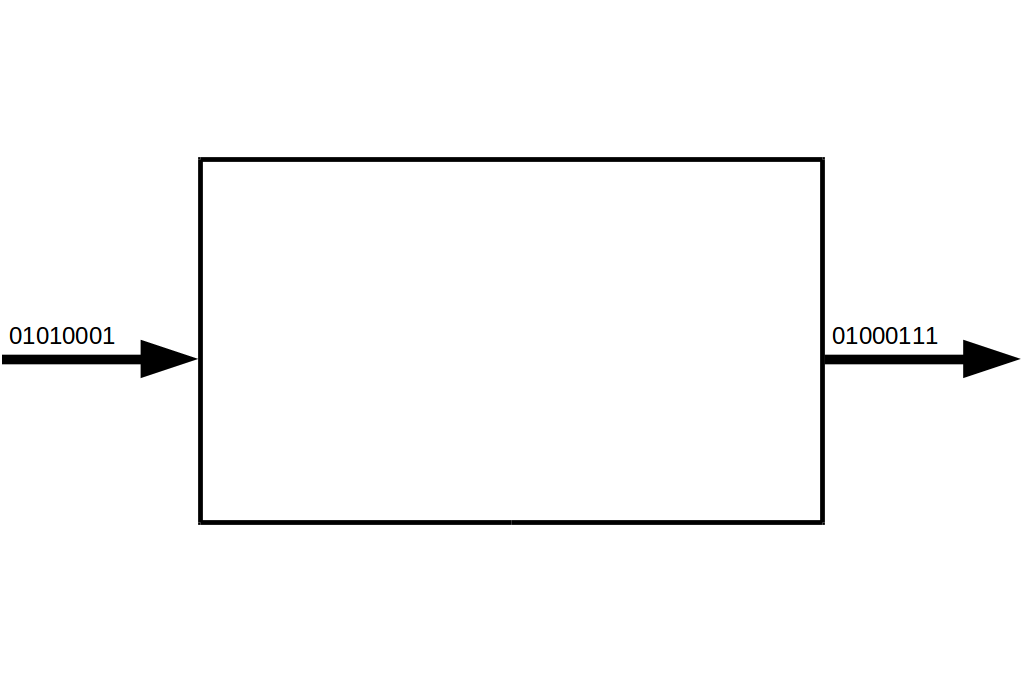
\includegraphics[width=0.9\linewidth]{../../img/cpu_blackbox_white} \end{center}
\end{frame}

\begin{frame}
\begin{center}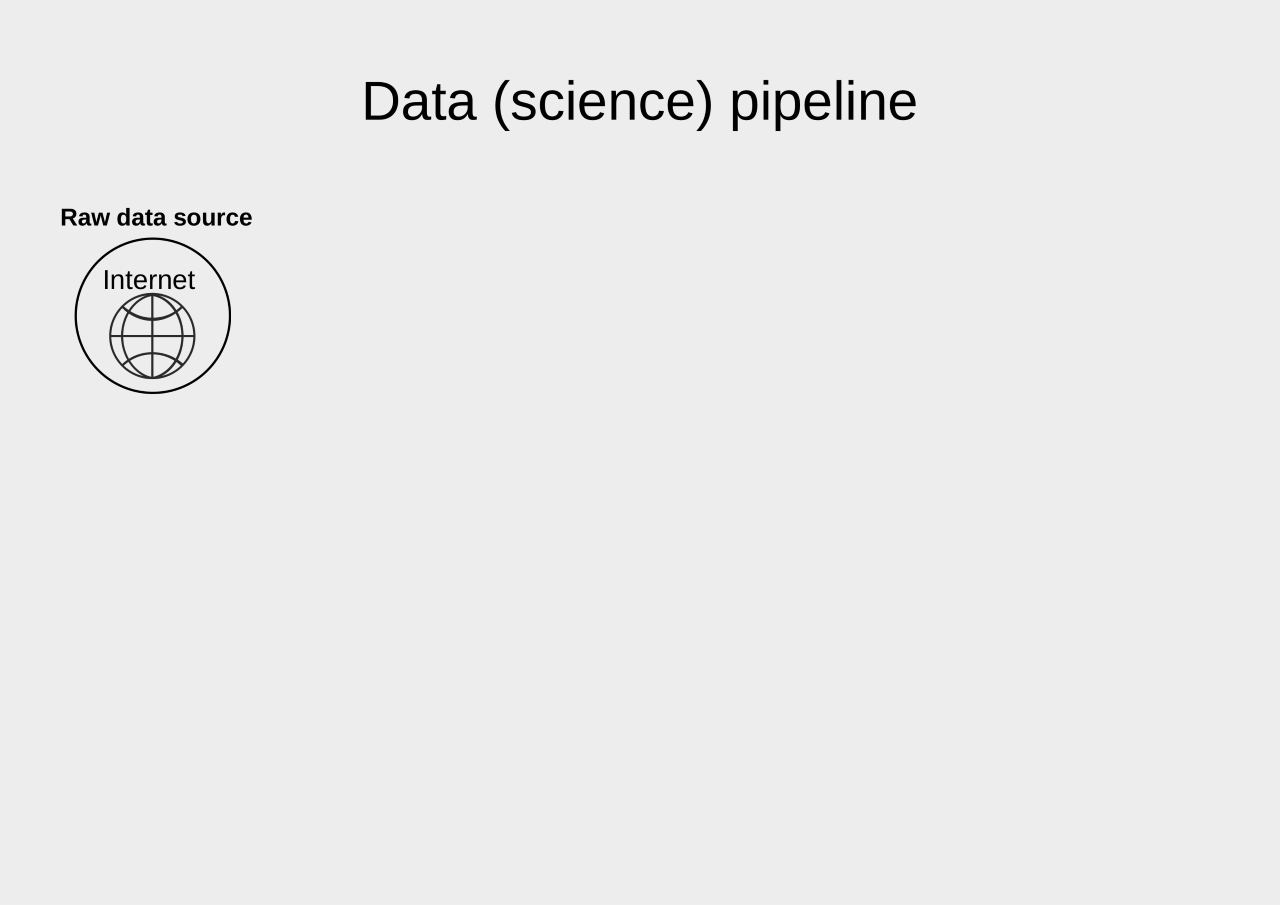
\includegraphics[width=0.9\linewidth]{../../img/ds1} \end{center}
\end{frame}

\begin{frame}
\begin{center}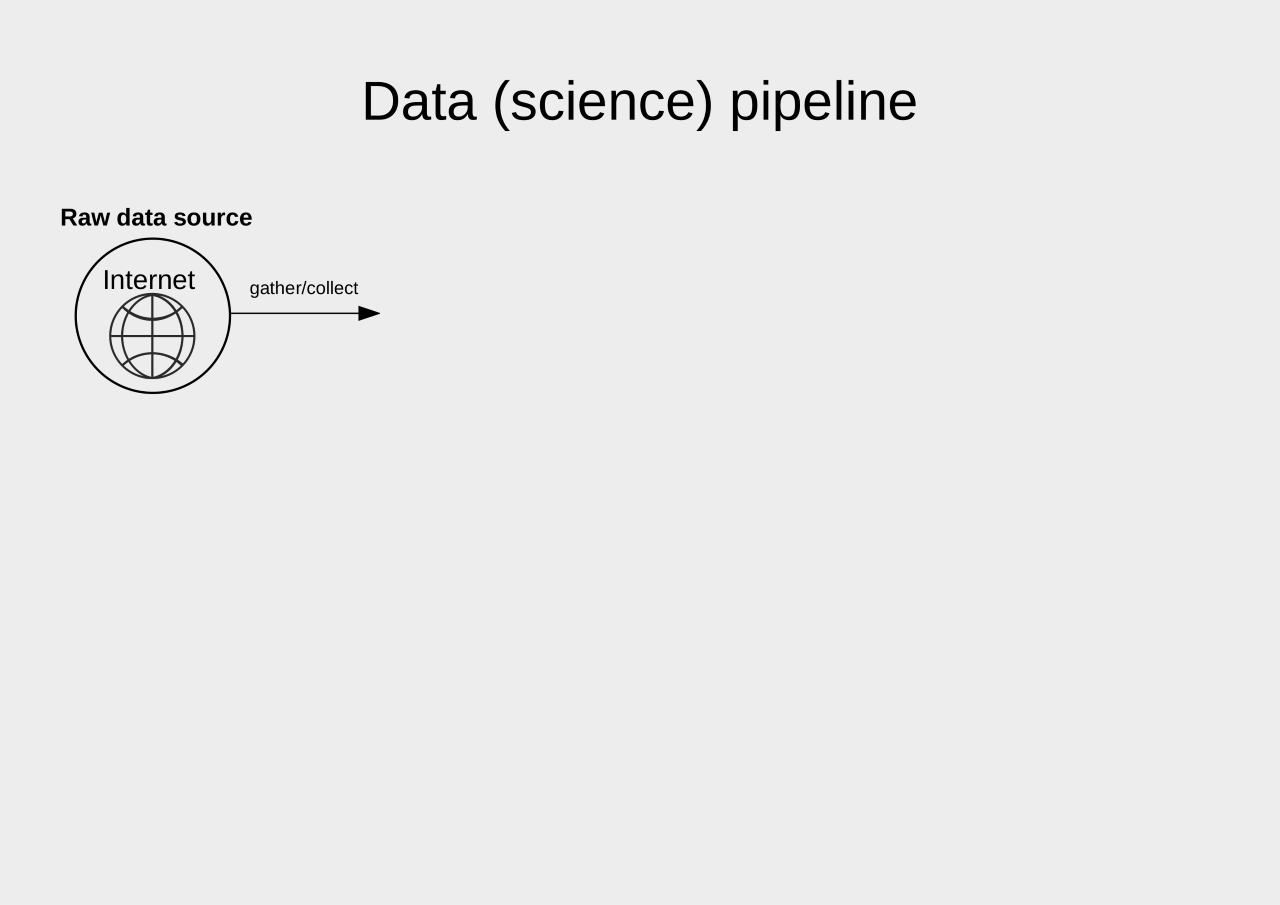
\includegraphics[width=0.9\linewidth]{../../img/ds2} \end{center}
\end{frame}

\begin{frame}
\begin{center}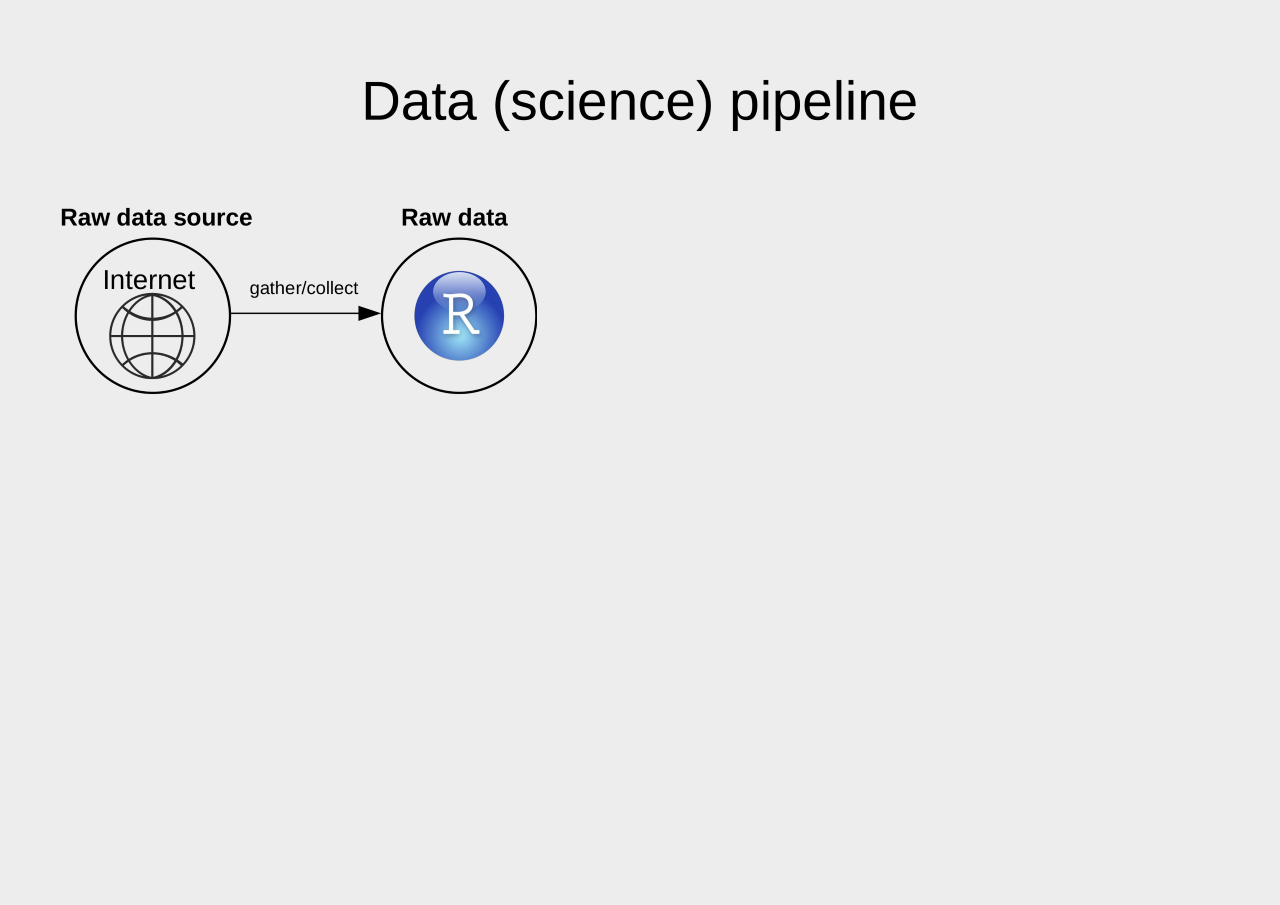
\includegraphics[width=0.9\linewidth]{../../img/ds3} \end{center}
\end{frame}

\begin{frame}
\begin{center}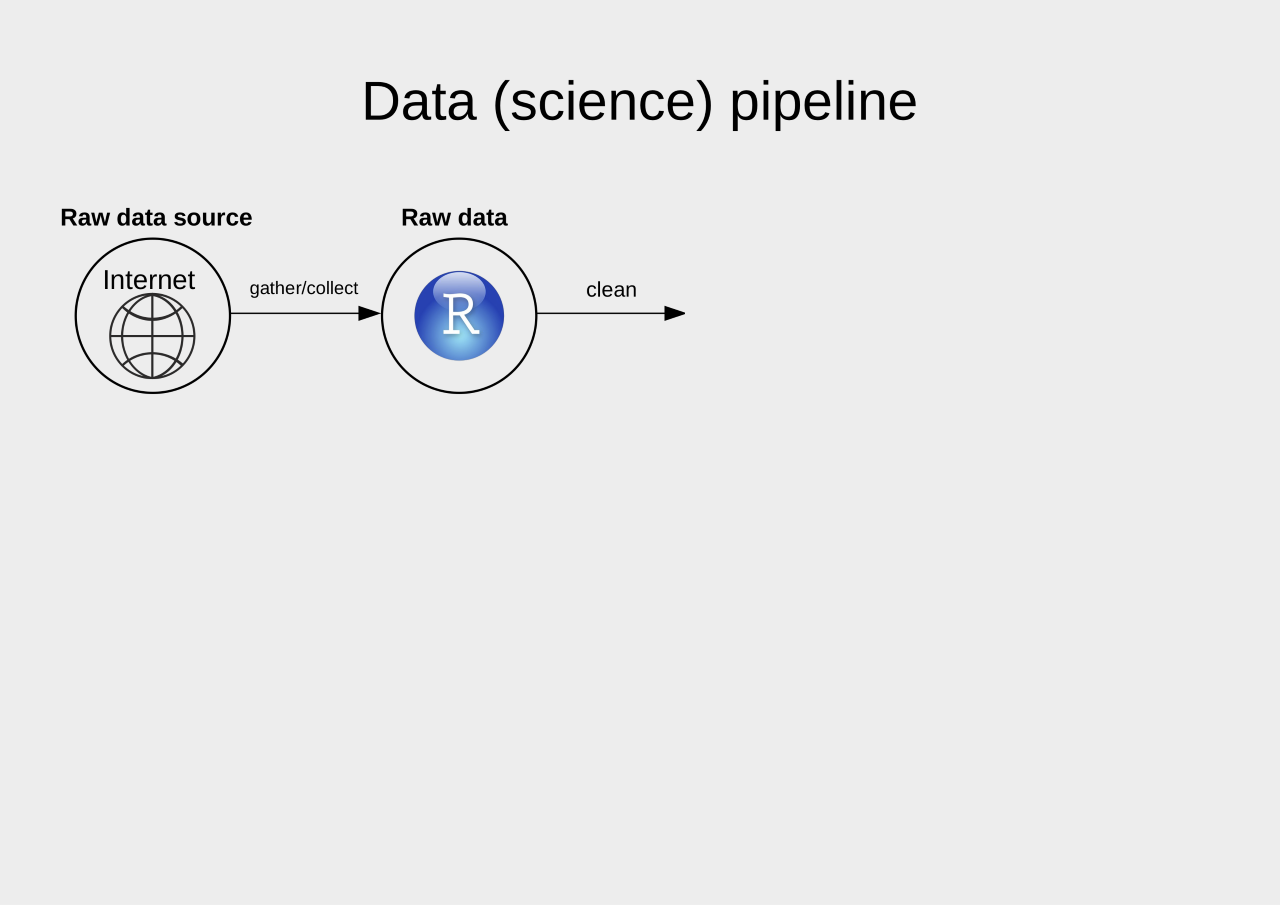
\includegraphics[width=0.9\linewidth]{../../img/ds4} \end{center}
\end{frame}

\begin{frame}
\begin{center}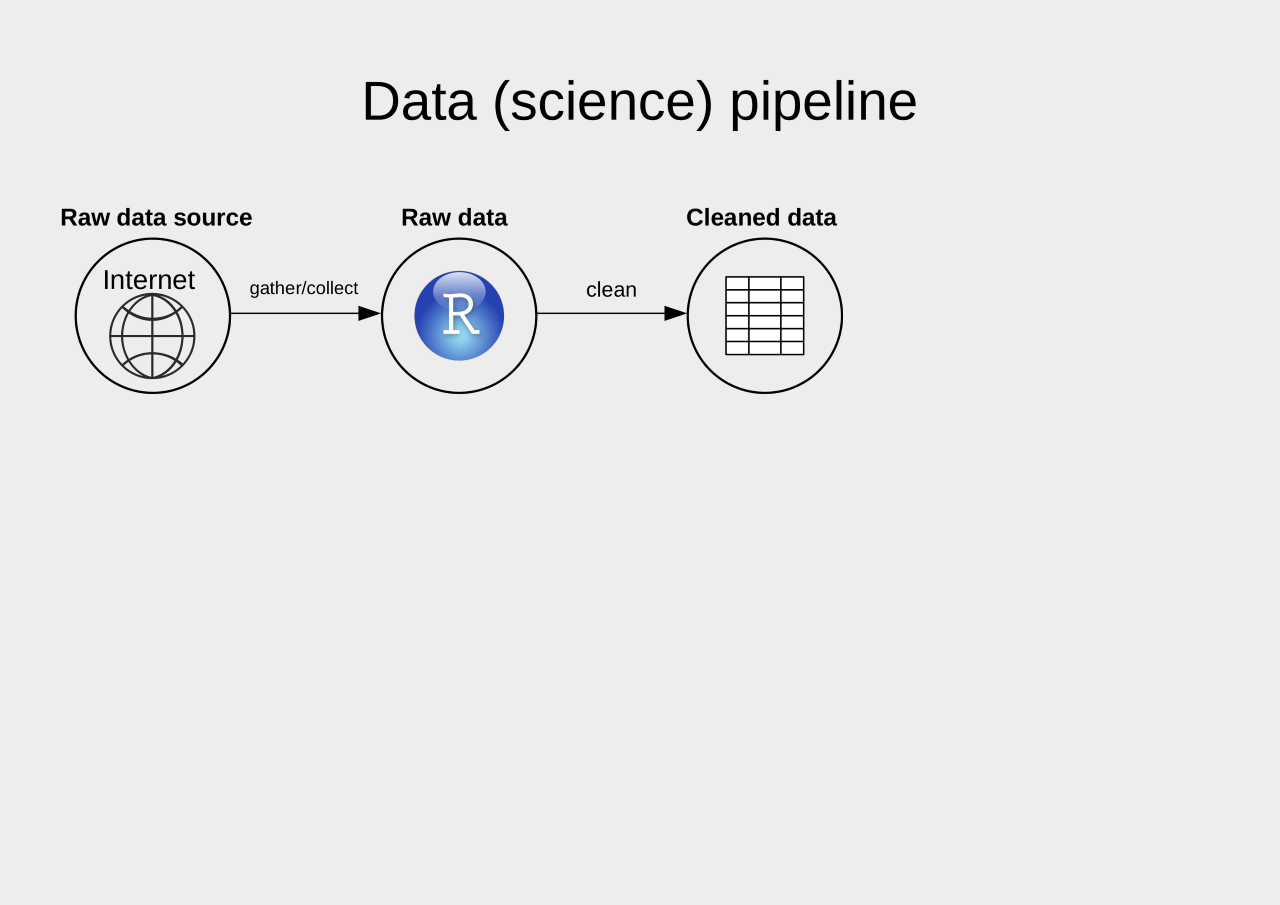
\includegraphics[width=0.9\linewidth]{../../img/ds5} \end{center}
\end{frame}

\begin{frame}
\begin{center}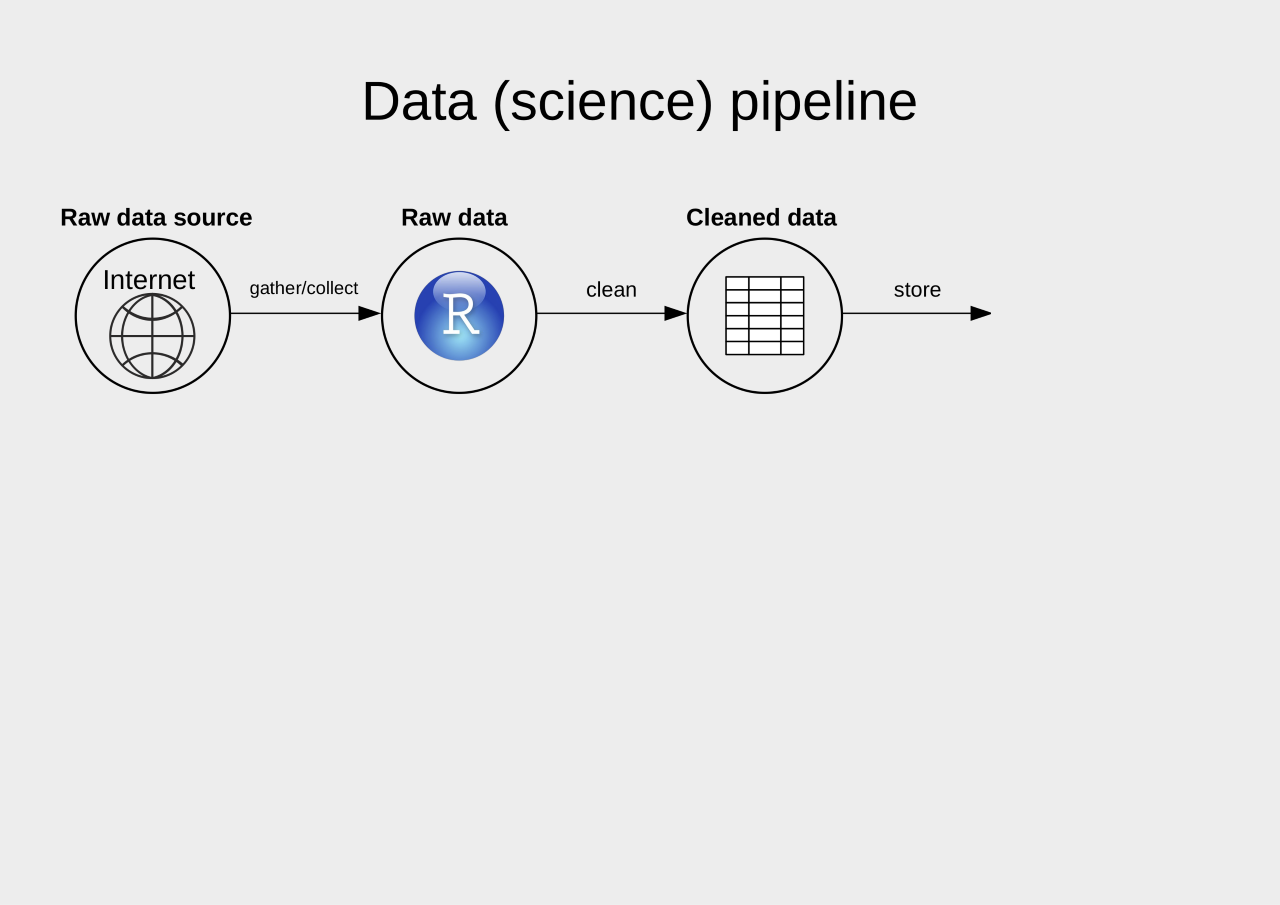
\includegraphics[width=0.9\linewidth]{../../img/ds6} \end{center}
\end{frame}

\begin{frame}
\begin{center}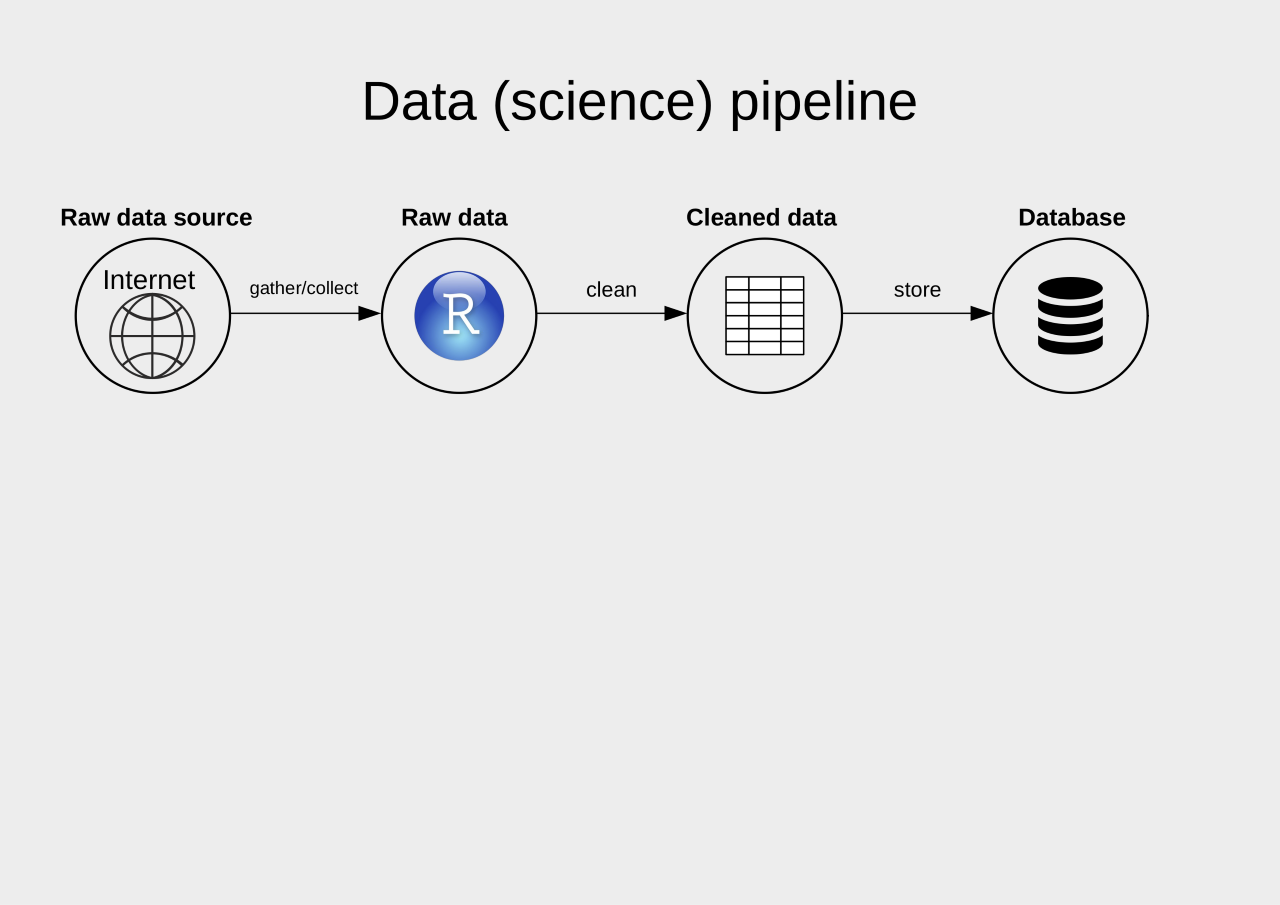
\includegraphics[width=0.9\linewidth]{../../img/ds7} \end{center}
\end{frame}

\begin{frame}
\begin{center}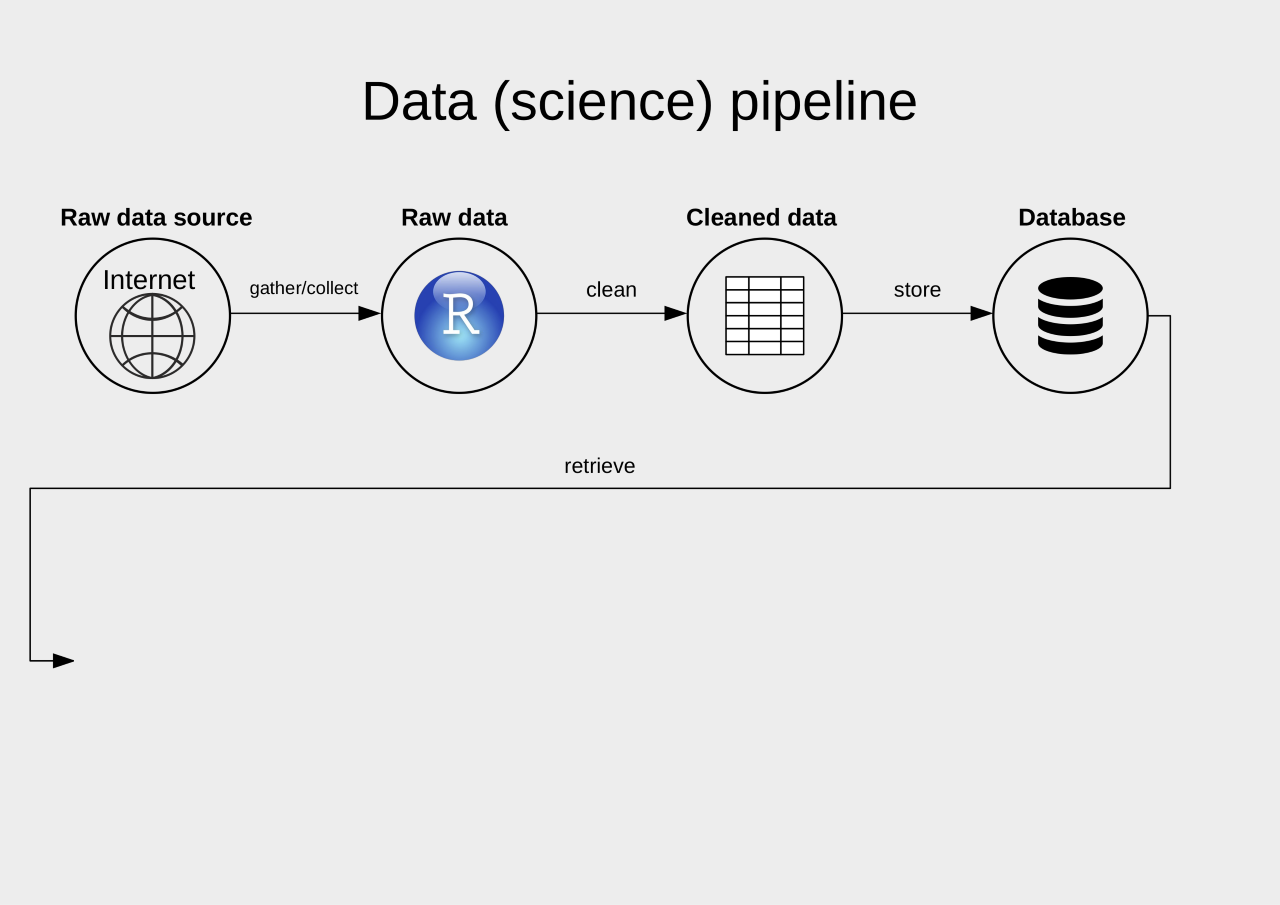
\includegraphics[width=0.9\linewidth]{../../img/ds8} \end{center}
\end{frame}

\begin{frame}
\begin{center}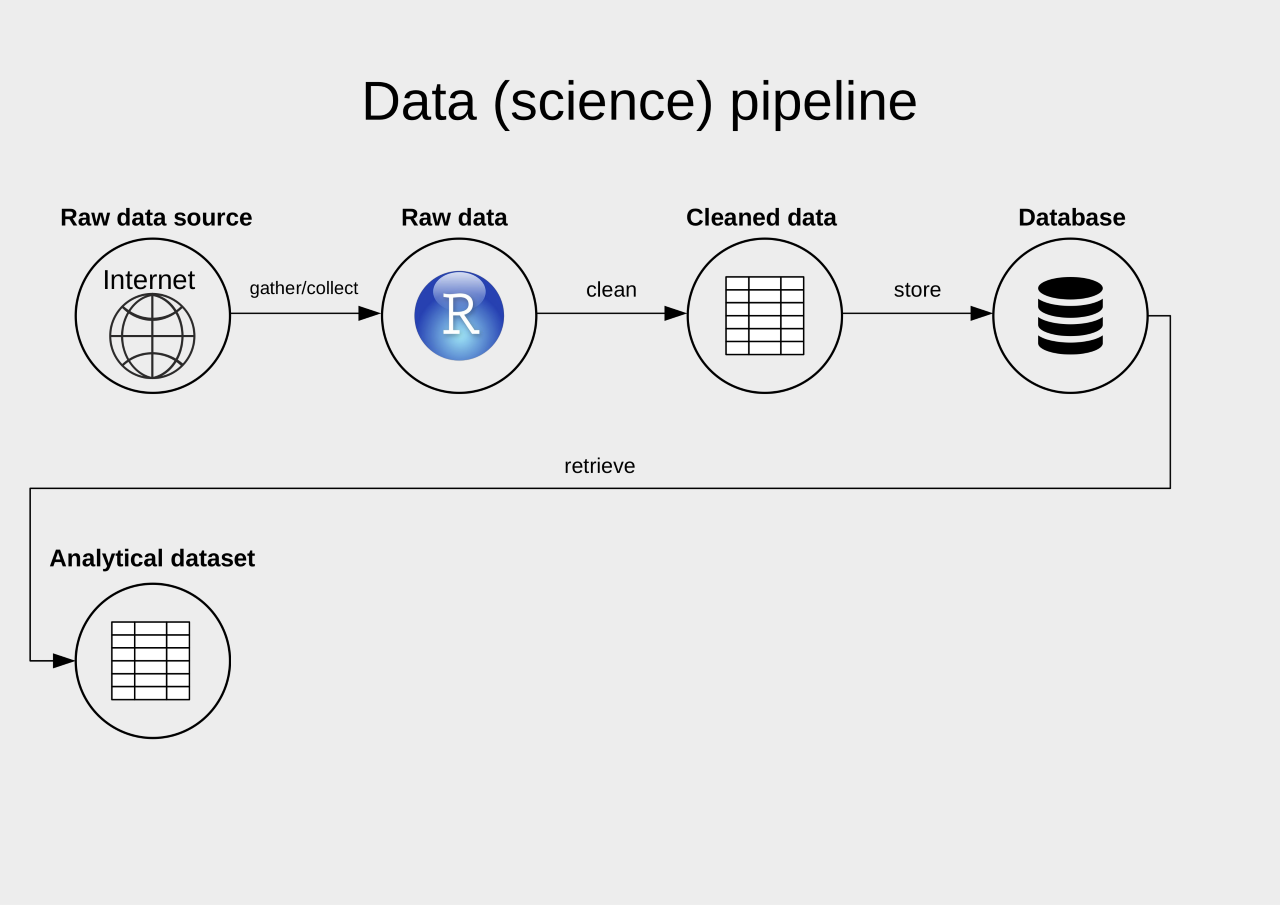
\includegraphics[width=0.9\linewidth]{../../img/ds9} \end{center}
\end{frame}

\begin{frame}
\begin{center}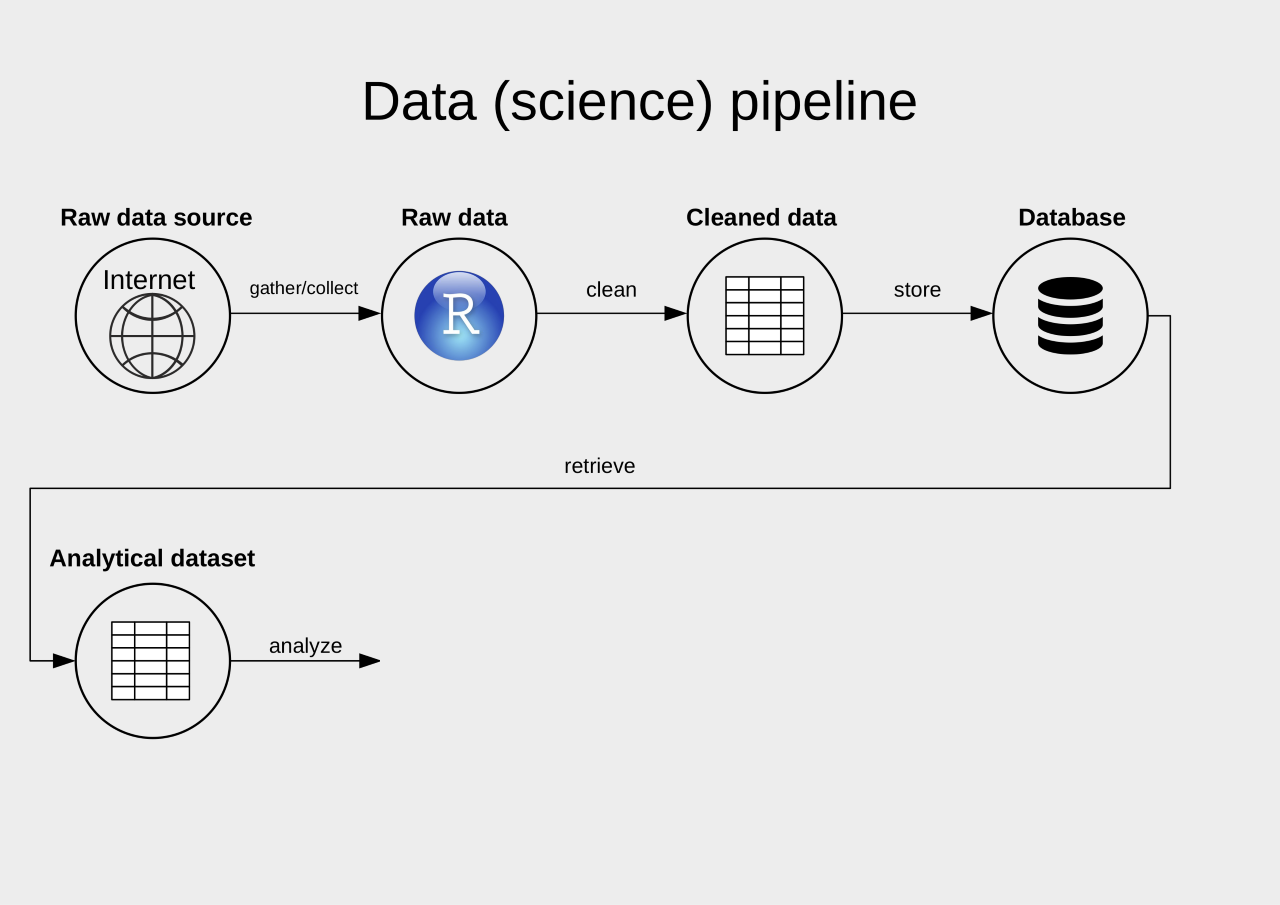
\includegraphics[width=0.9\linewidth]{../../img/ds10} \end{center}
\end{frame}

\begin{frame}
\begin{center}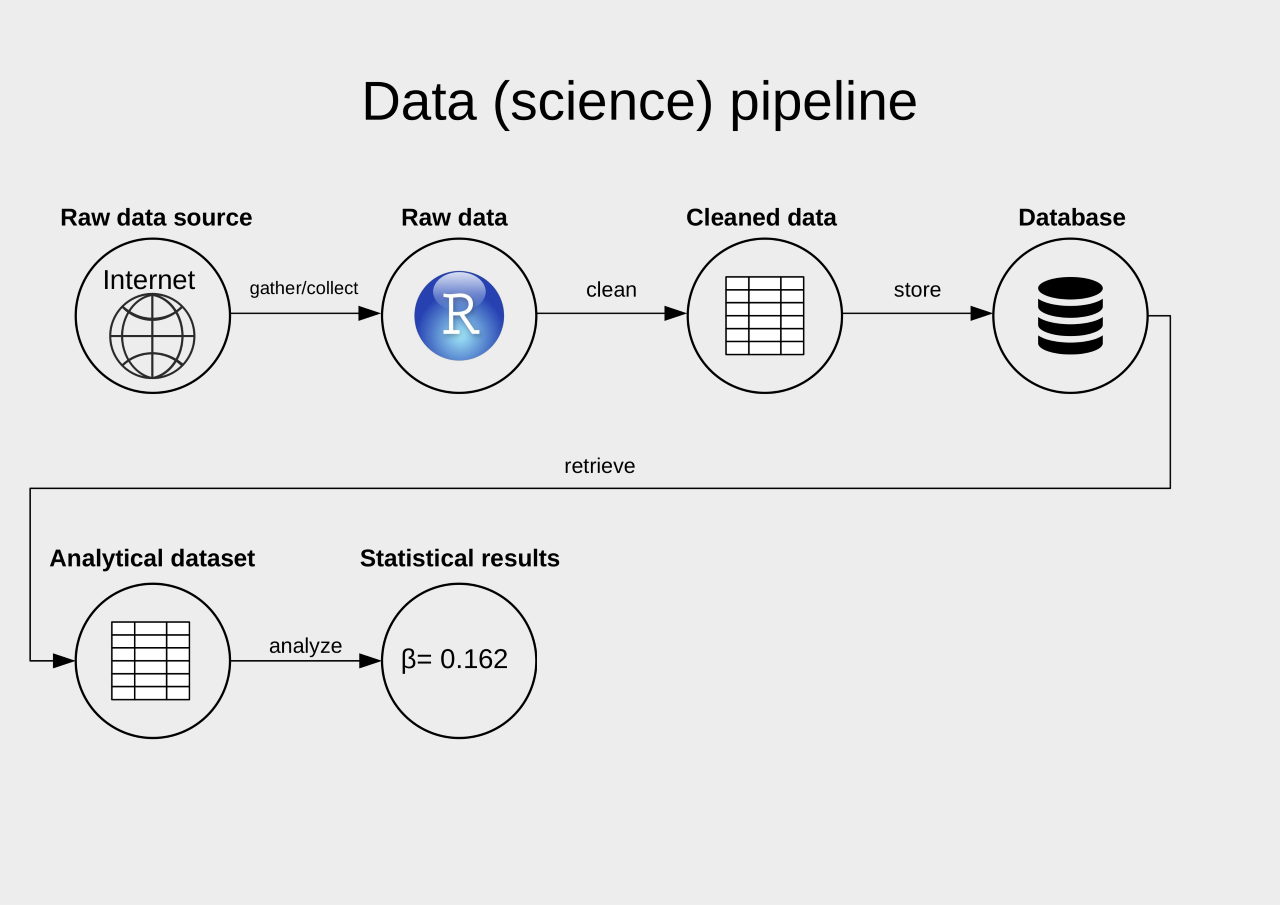
\includegraphics[width=0.9\linewidth]{../../img/ds11} \end{center}
\end{frame}

\begin{frame}
\begin{center}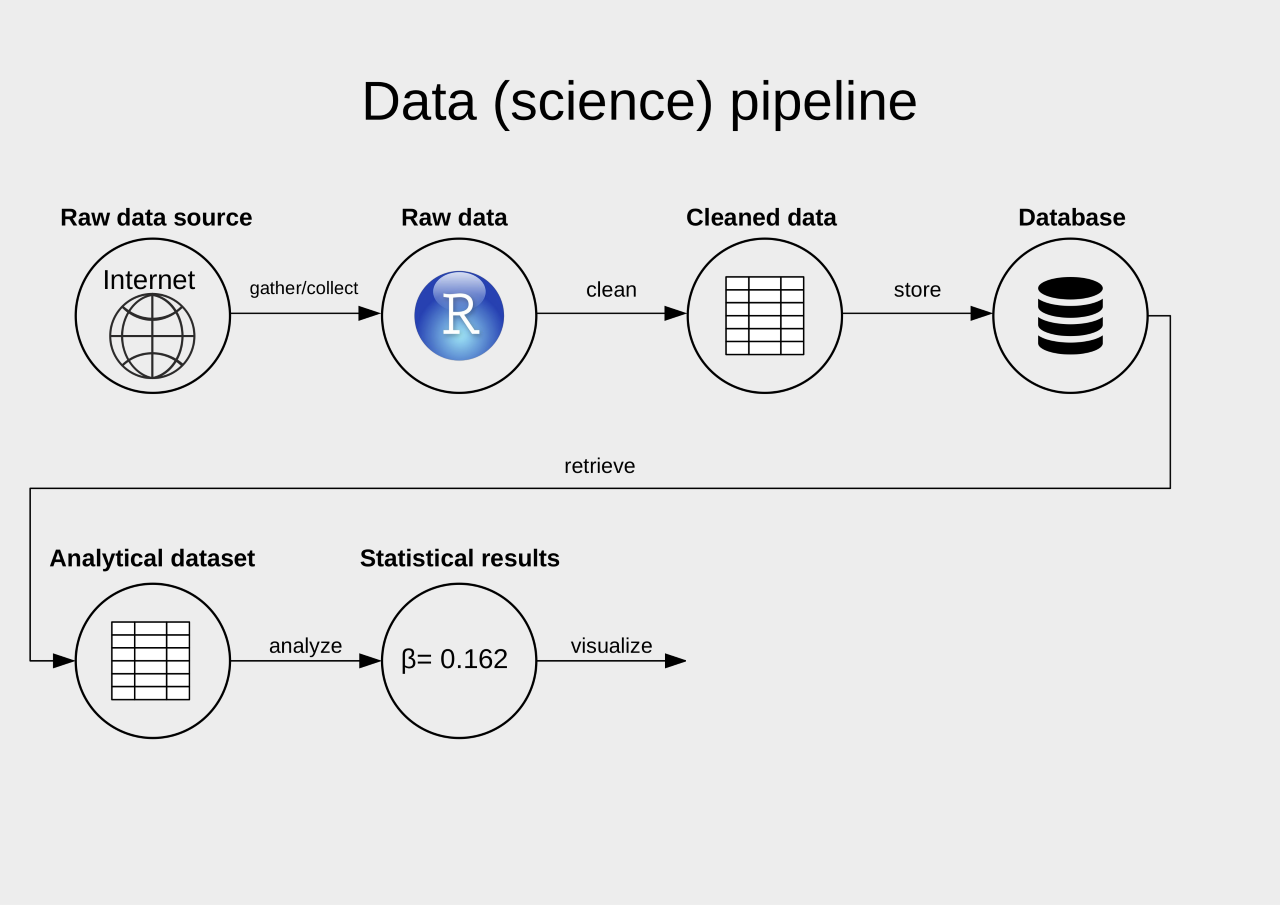
\includegraphics[width=0.9\linewidth]{../../img/ds12} \end{center}
\end{frame}

\begin{frame}
\begin{center}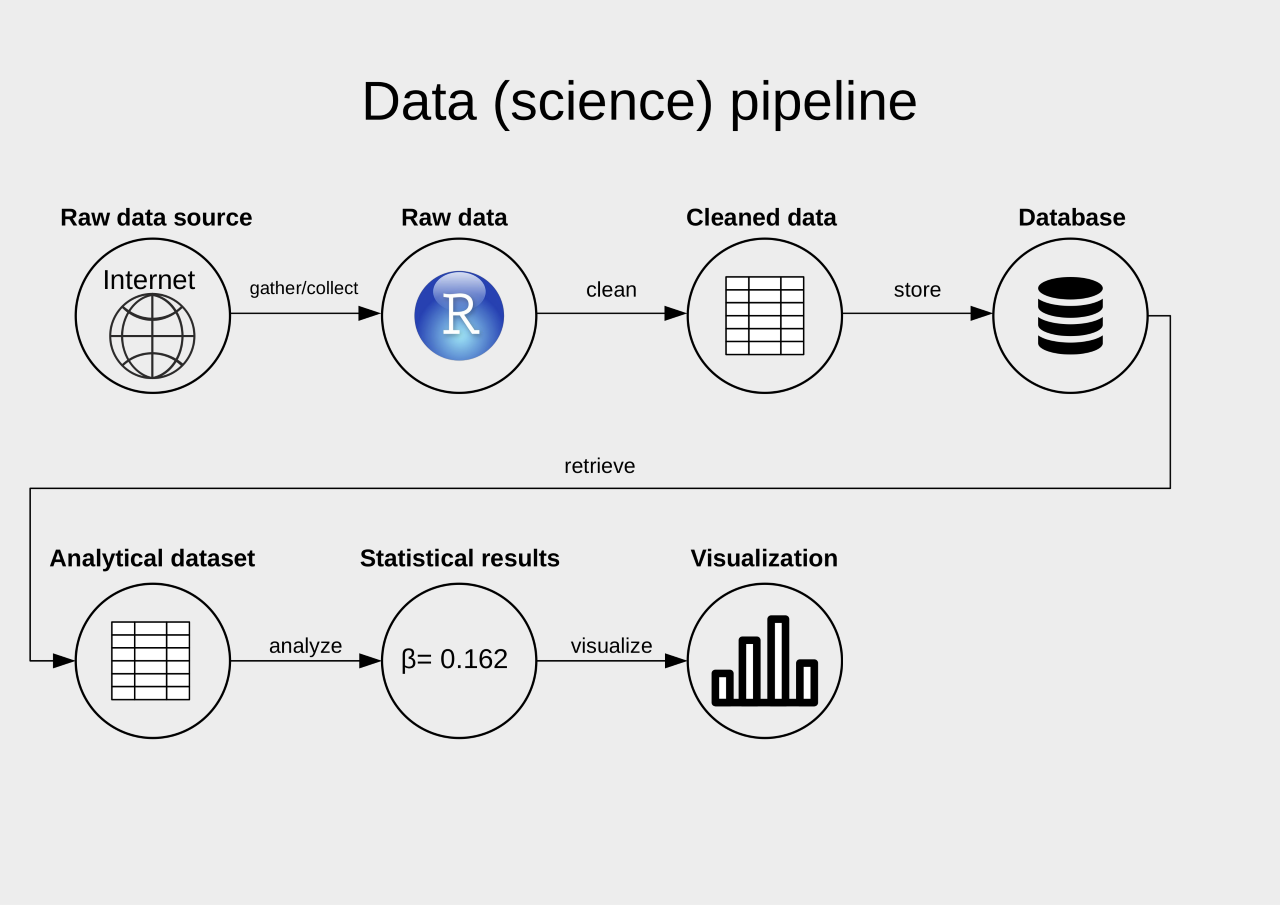
\includegraphics[width=0.9\linewidth]{../../img/ds13} \end{center}
\end{frame}

\begin{frame}
\begin{center}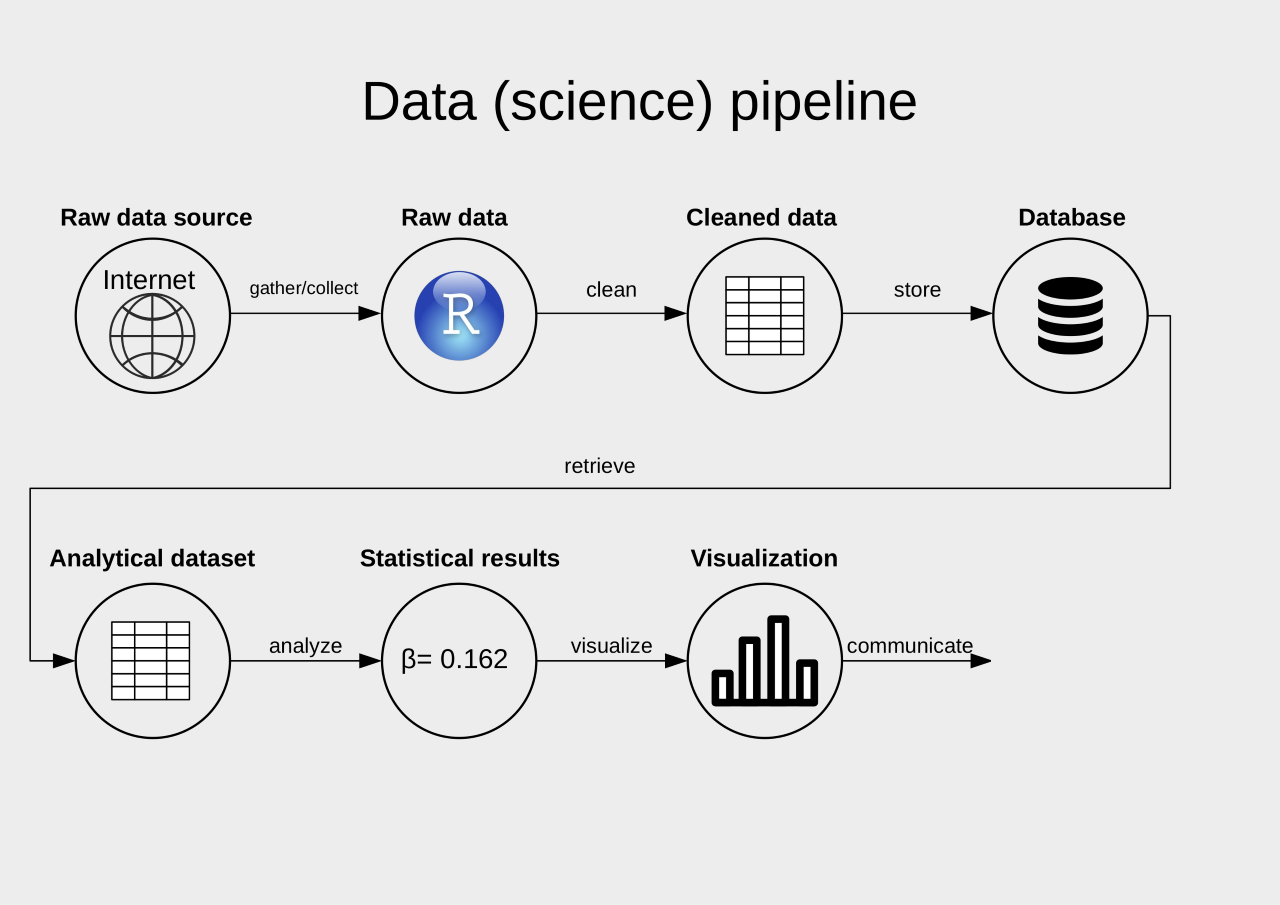
\includegraphics[width=0.9\linewidth]{../../img/ds14} \end{center}
\end{frame}

\begin{frame}
\begin{center}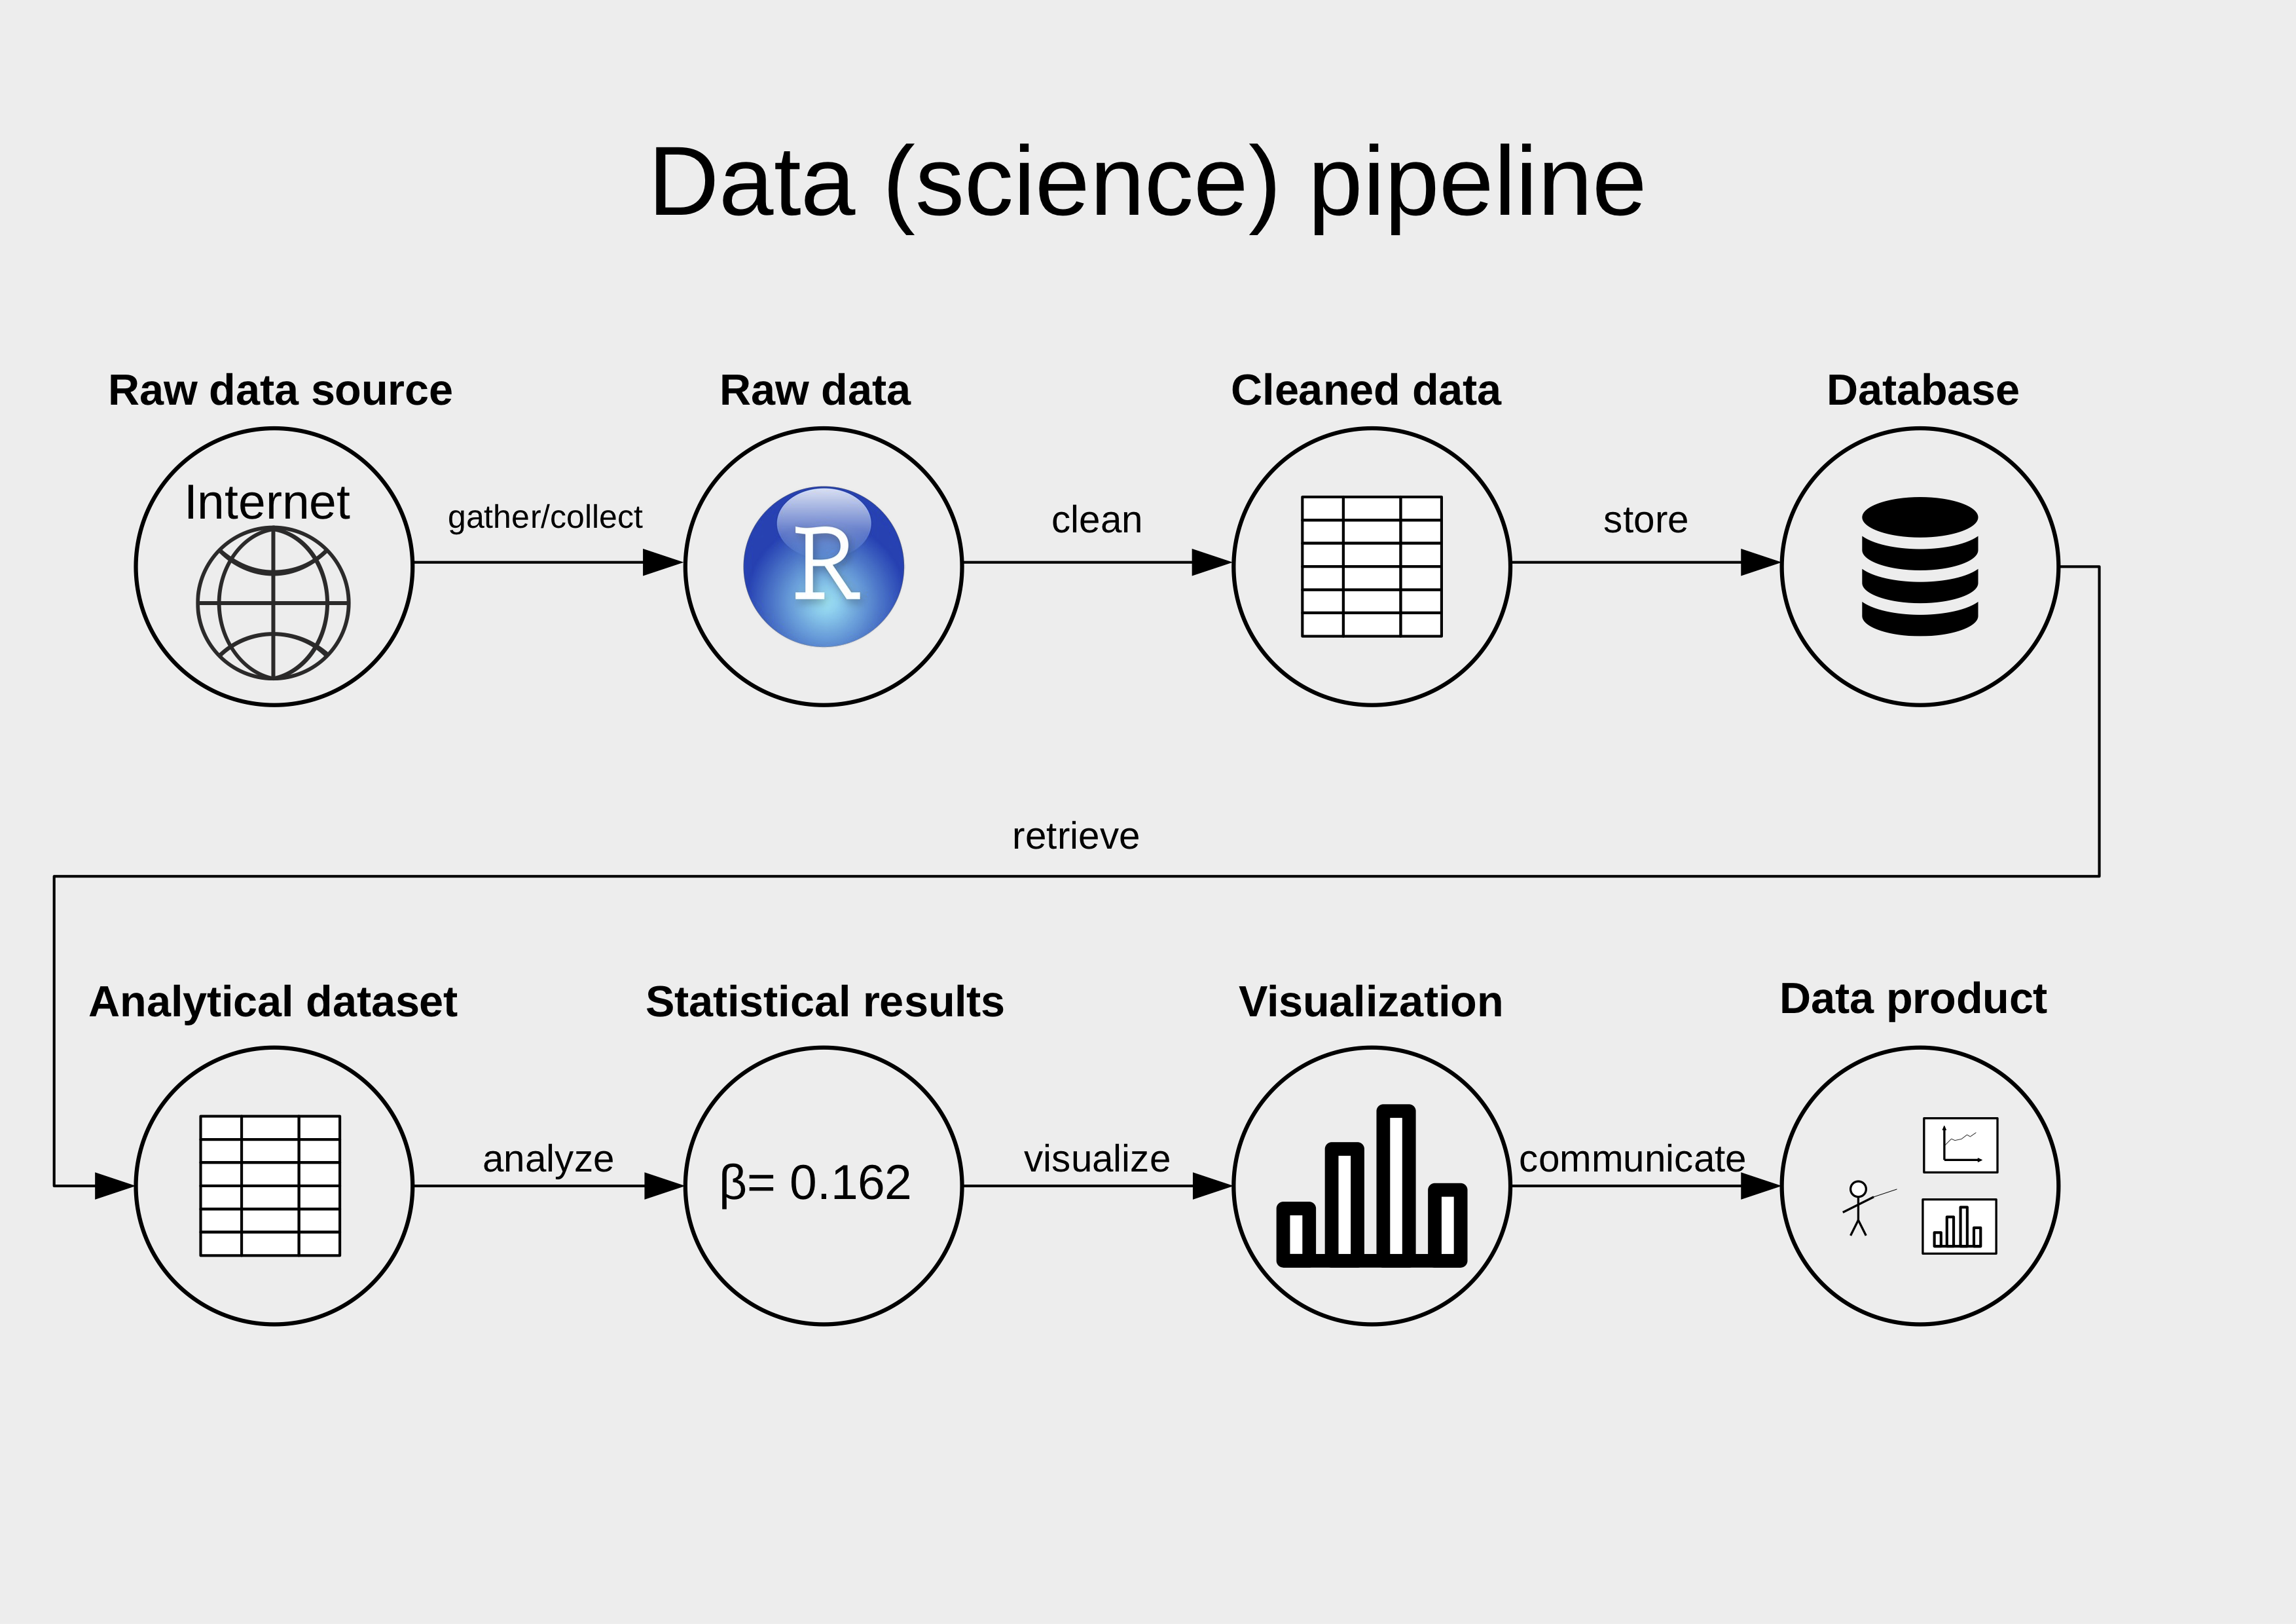
\includegraphics[width=0.9\linewidth]{../../img/data_science_pipeline} \end{center}
\end{frame}

\begin{frame}{Background}
\protect\hypertarget{background}{}
\begin{block}{`Data Science'?}
\protect\hypertarget{data-science}{}
\emph{``This coupling of scientific discovery and practice involves the
collection, management, processing, analysis, visualization, and
interpretation of vast amounts of heterogeneous data associated with a
diverse array of scientific, translational, and inter-disciplinary
applications.''}

University of Michigan `Data Science Initiative', 2015
\end{block}

\begin{block}{But, what about statistics?!}
\protect\hypertarget{but-what-about-statistics}{}
\emph{``Seemingly, statistics is being marginalized here; the implicit
message is that statistics is a part of what goes on in data science but
not a very big part. At the same time, many of the concrete descriptions
of what the DSI will actually do will seem to statisticians to be
bread-and-butter statistics. Statistics is apparently the word that dare
not speak its name in connection with such an initiative!''}

David Donoho (2015). \textbf{50 years of Data Science}
\end{block}

\begin{block}{What's new about all this?}
\protect\hypertarget{whats-new-about-all-this}{}
\emph{``All in all, I have come to feel that my central interest is in
data analysis, which I take to include, among other things: \ldots{}''}
\end{block}

\begin{block}{What's new about all this?}
\protect\hypertarget{whats-new-about-all-this-1}{}
\emph{``All in all, I have come to feel that my central interest is in
data analysis, which I take to include, among other things: procedures
for analyzing data, techniques for interpreting the results of such
procedures, ways of planning the gathering of data to make its analysis
easier, more precise or more accurate, and all the machinery and results
of (mathematical) statistics which apply to analyzing data.''}
\end{block}

\begin{block}{What's new about all this?}
\protect\hypertarget{whats-new-about-all-this-2}{}
\begin{center}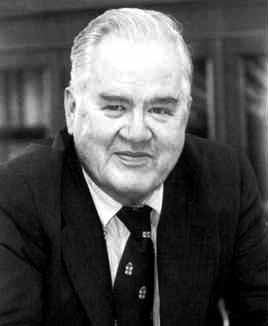
\includegraphics[width=0.4\linewidth]{../../img/tukey} \end{center}

John Tukey (\emph{The Future of Data Analysis}, 1962!)
\end{block}

\begin{block}{Technological change}
\protect\hypertarget{technological-change}{}
\begin{center}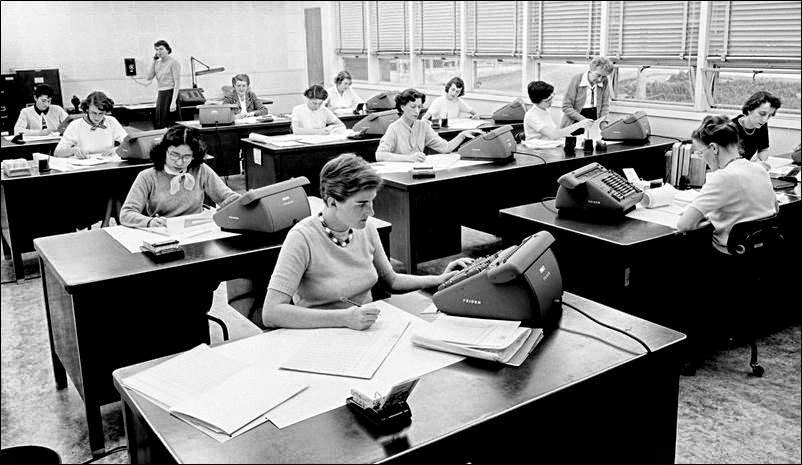
\includegraphics[width=0.9\linewidth]{../../img/computers} \end{center}
\end{block}

\begin{block}{Relevance for modern economic research}
\protect\hypertarget{relevance-for-modern-economic-research}{}
\begin{center}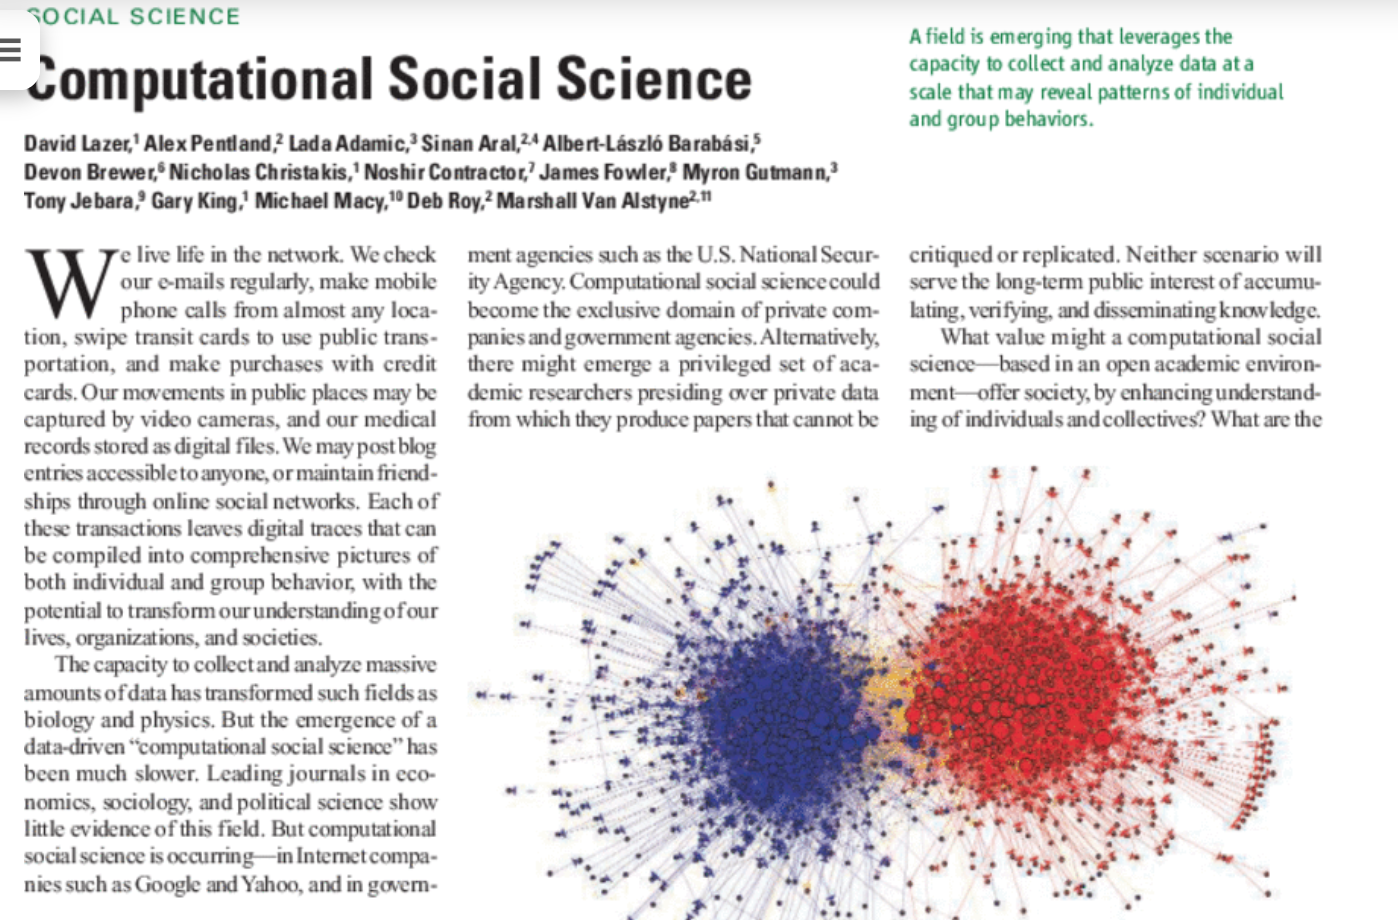
\includegraphics[width=0.9\linewidth]{../../img/css} \end{center}
\end{block}

\begin{block}{Relevance for modern economic research}
\protect\hypertarget{relevance-for-modern-economic-research-1}{}
\begin{center}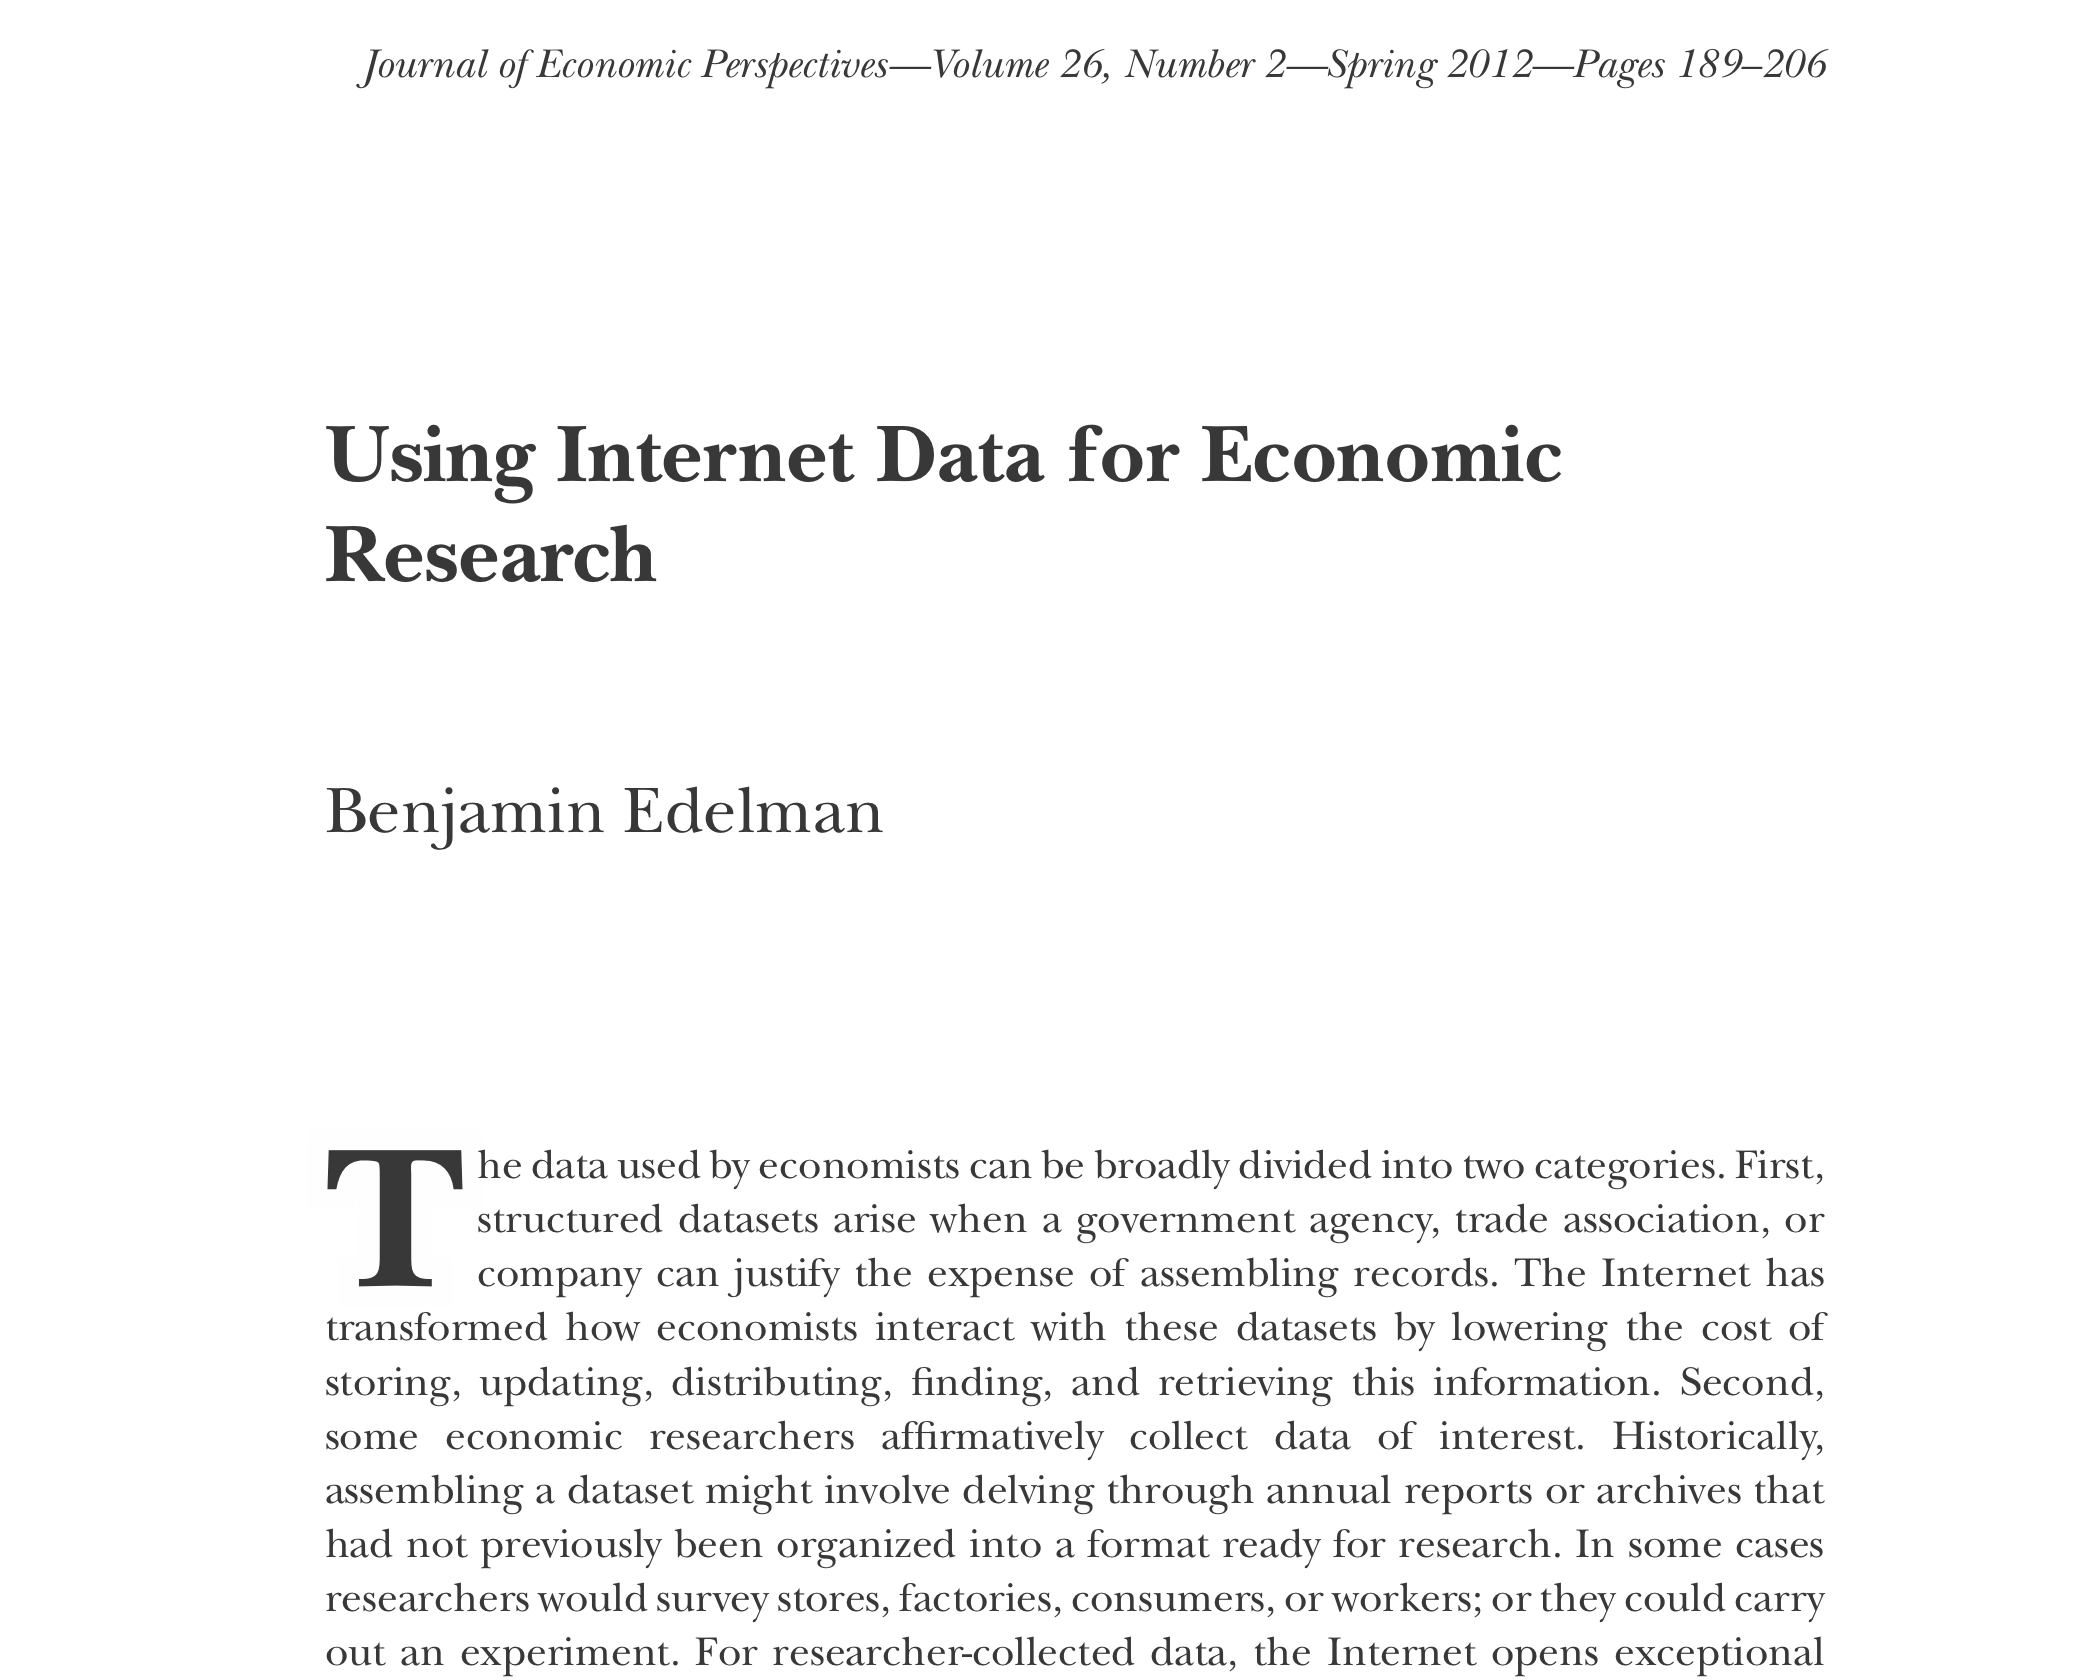
\includegraphics[width=0.9\linewidth]{../../img/internet} \end{center}
\end{block}

\begin{block}{Relevance for modern economic research}
\protect\hypertarget{relevance-for-modern-economic-research-2}{}
\begin{center}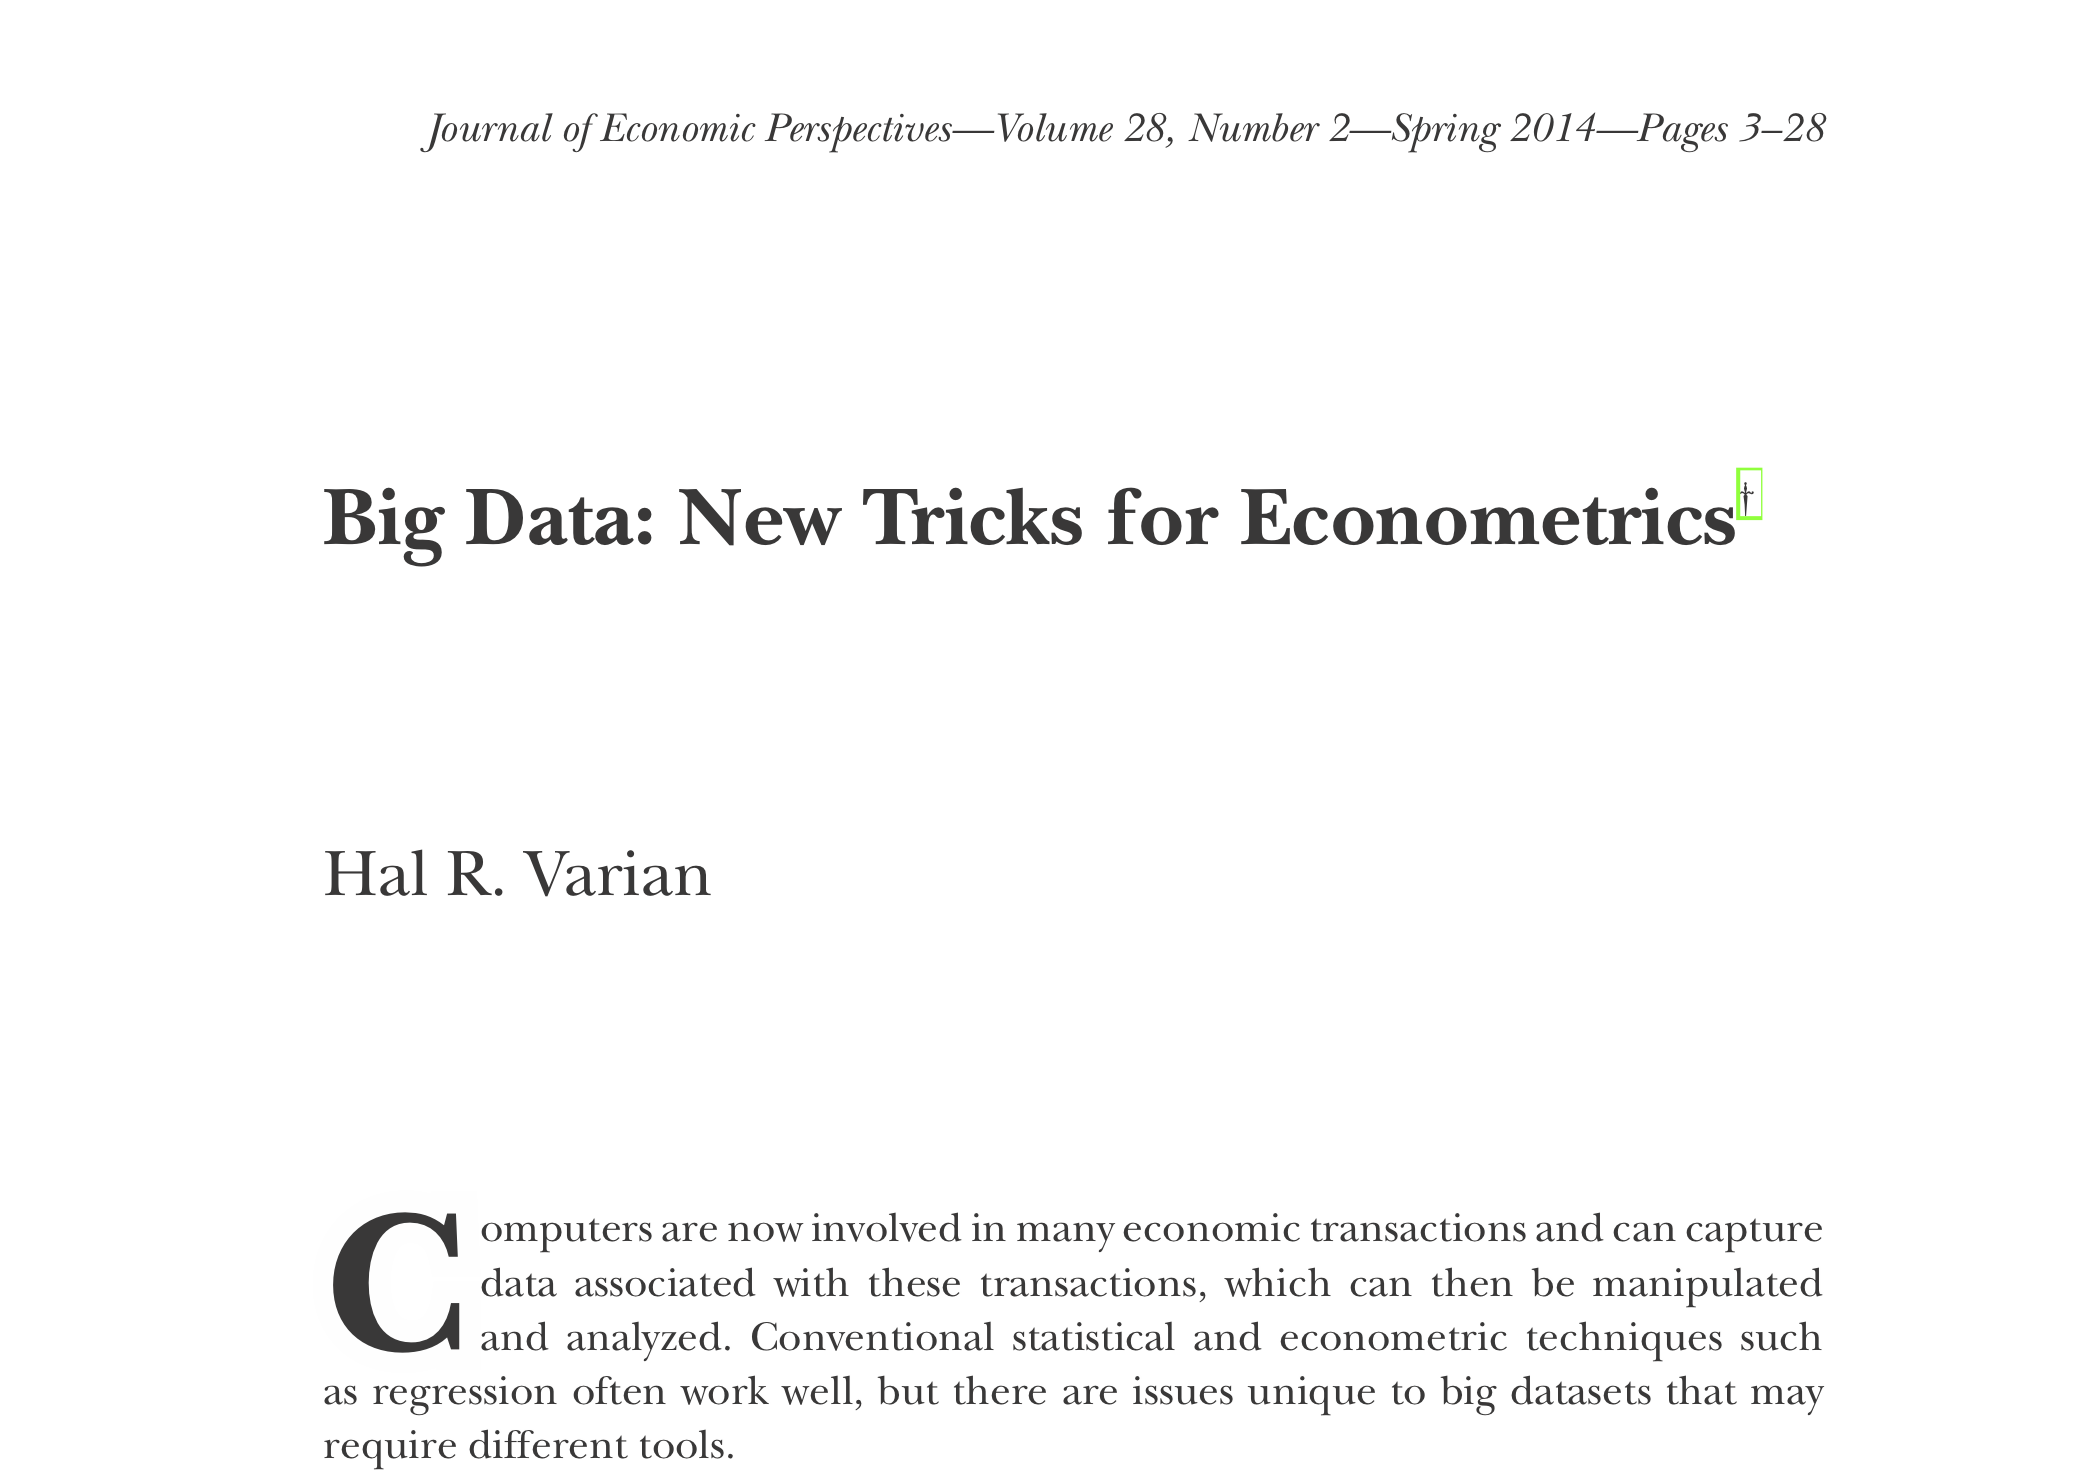
\includegraphics[width=0.9\linewidth]{../../img/bigdata} \end{center}
\end{block}

\begin{block}{Relevance for modern economic research}
\protect\hypertarget{relevance-for-modern-economic-research-3}{}
\begin{center}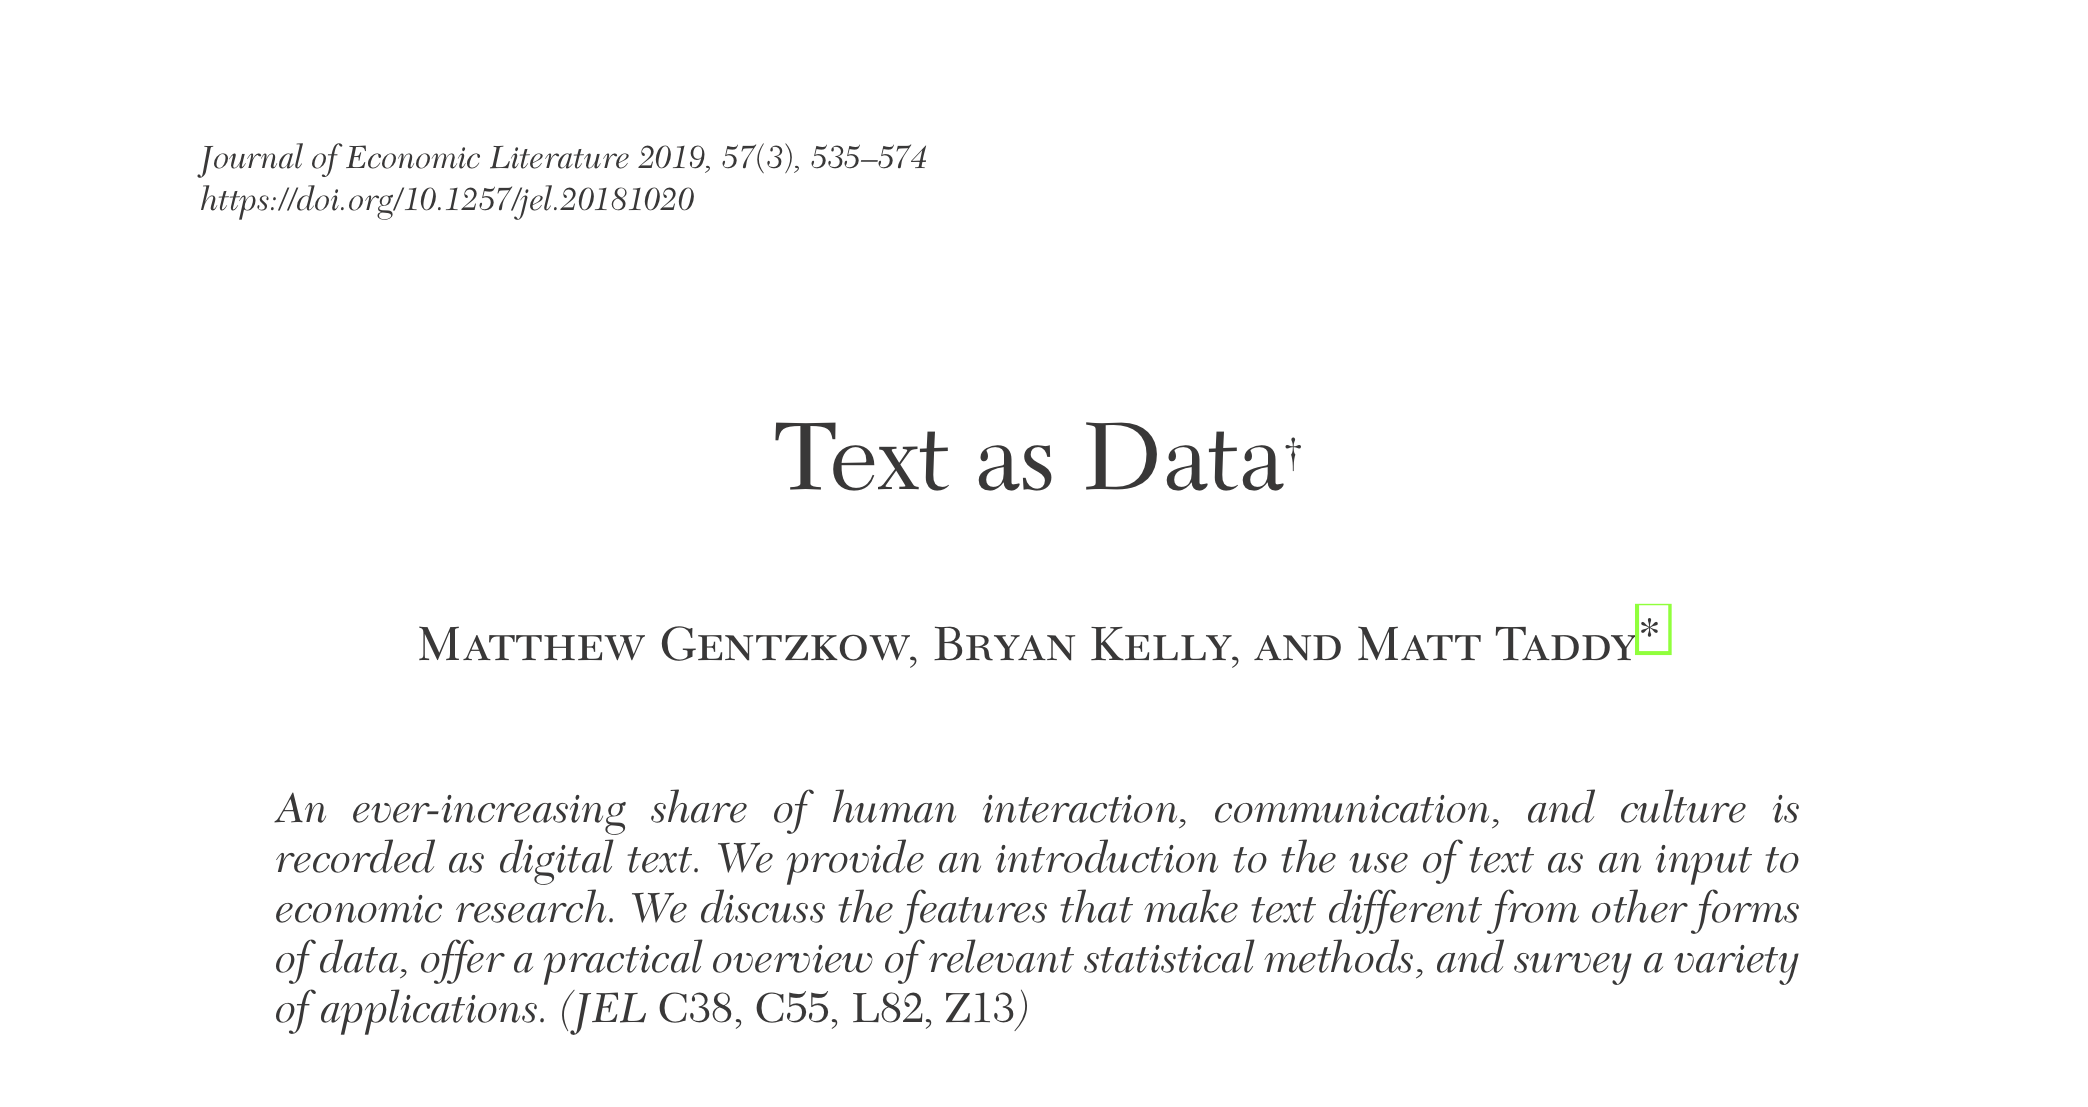
\includegraphics[width=0.9\linewidth]{../../img/text} \end{center}
\end{block}

\begin{block}{Data science in economics skill set}
\protect\hypertarget{data-science-in-economics-skill-set}{}
\begin{center}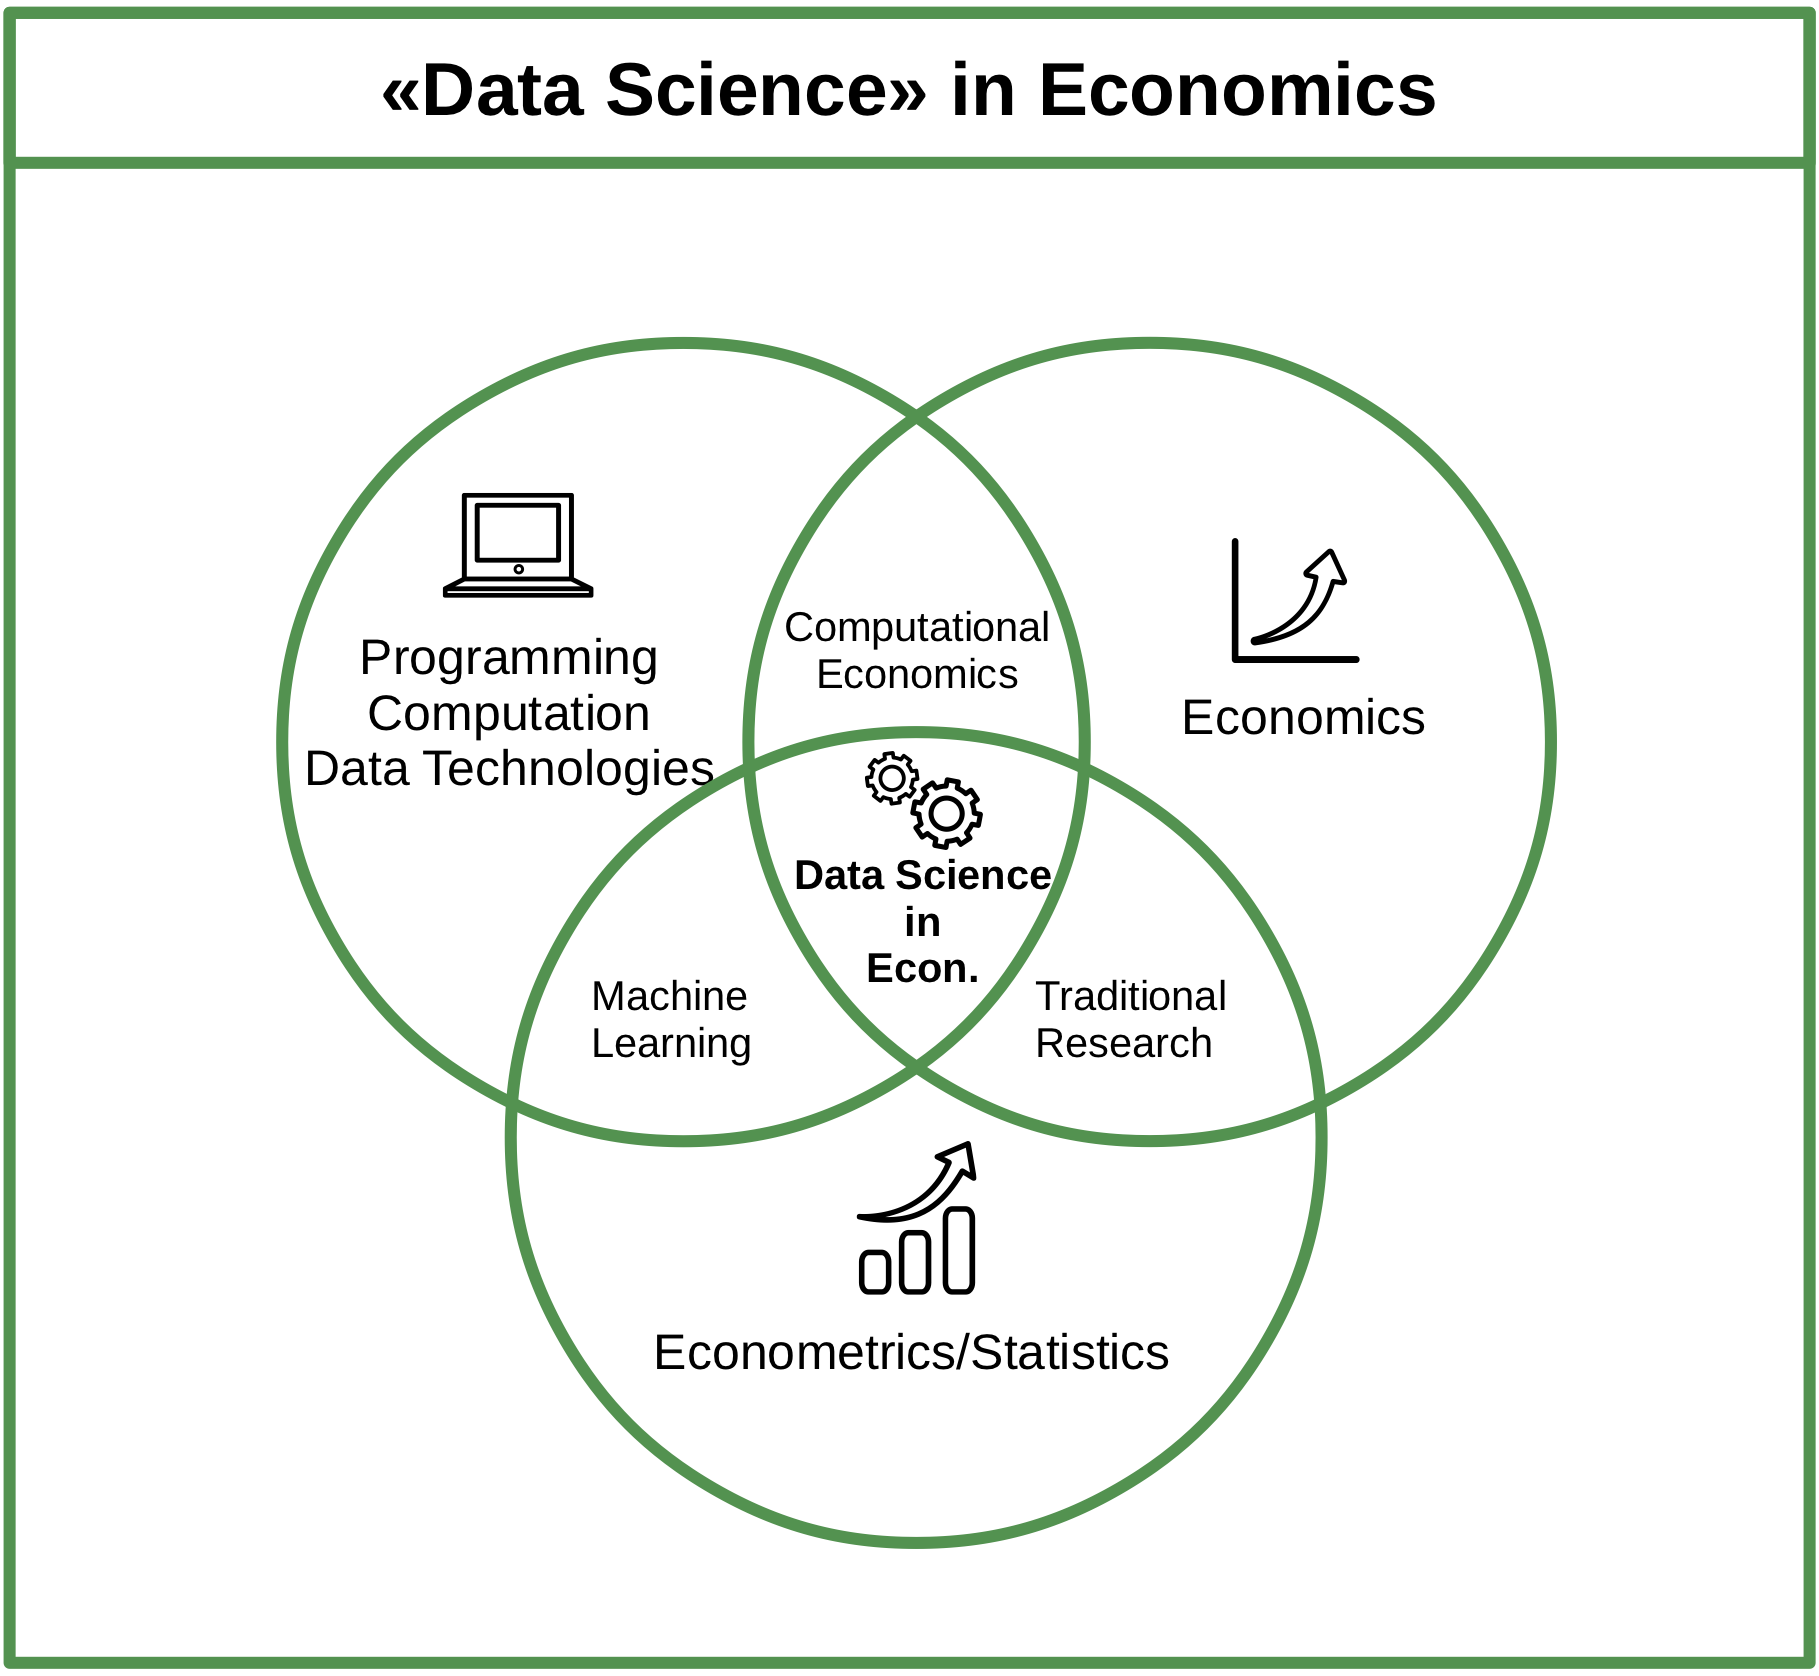
\includegraphics[width=0.6\linewidth]{../../img/venn_diagramm} \end{center}
\end{block}

\begin{block}{Data science as a life skill}
\protect\hypertarget{data-science-as-a-life-skill}{}
\begin{center}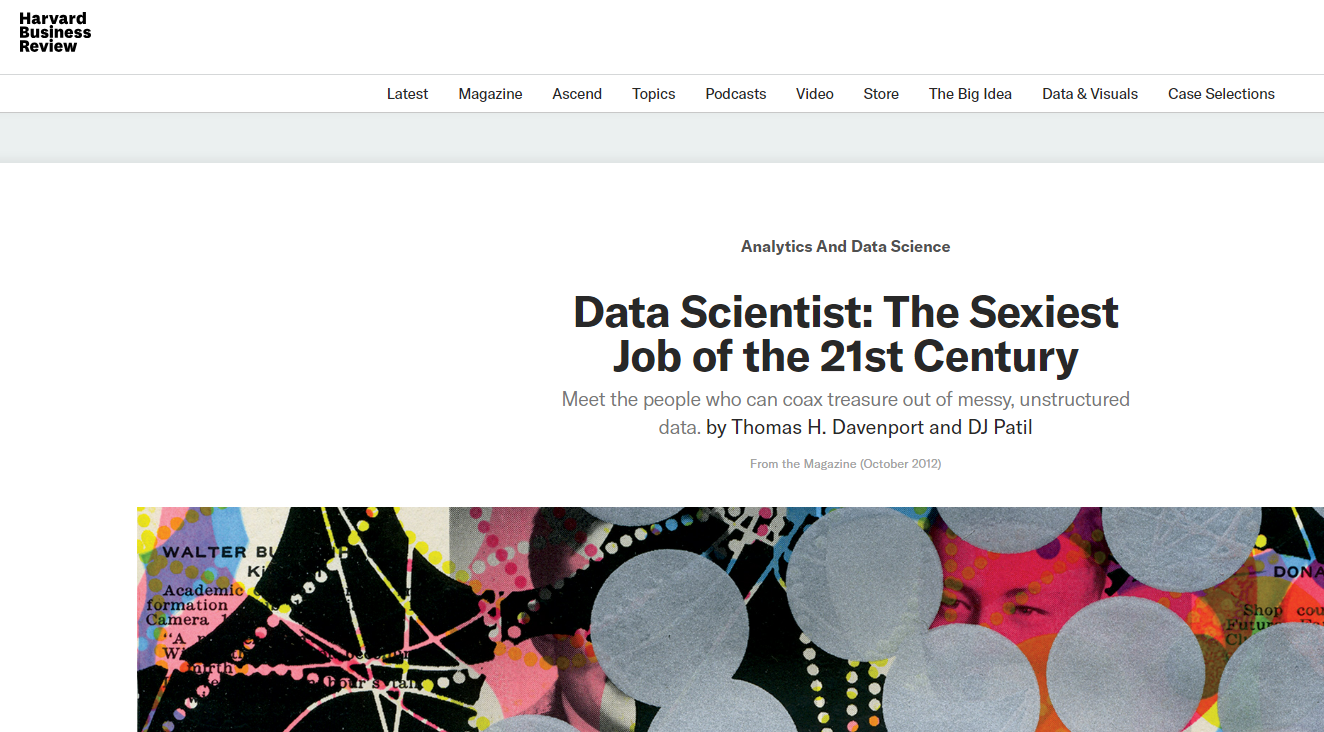
\includegraphics[width=0.8\linewidth]{../../img/datascientistsexy} \end{center}
\end{block}

\begin{block}{Data science as a life skill}
\protect\hypertarget{data-science-as-a-life-skill-1}{}
``More than anything, what data scientists do is \emph{make discoveries
while swimming in data.} \ldots{} As they make discoveries, they
communicate what they've learned and suggest its implications for new
business directions. Often they are \emph{creative in displaying
information visually and making the patterns they find clear and
compelling}\ldots{}

They advise executives and product managers on the implications of the
data for \emph{products, processes, and decisions}.

What kind of person does all this? \emph{Think of him or her as a hybrid
of data hacker, analyst, communicator, and trusted adviser. The
combination is extremely powerful --- and rare.}''
\end{block}
\end{frame}

\begin{frame}{Organisation of the Course}
\protect\hypertarget{organisation-of-the-course}{}
\begin{block}{Our Team - At Your Service}
\protect\hypertarget{our-team---at-your-service}{}
\begin{longtable}[]{@{}
  >{\raggedright\arraybackslash}p{(\columnwidth - 4\tabcolsep) * \real{0.2750}}
  >{\raggedright\arraybackslash}p{(\columnwidth - 4\tabcolsep) * \real{0.3625}}
  >{\raggedright\arraybackslash}p{(\columnwidth - 4\tabcolsep) * \real{0.3625}}@{}}
\toprule
\endhead
& & \\
Matthias Rösti & Andrea Burro & Aurélien Sallin \\
\bottomrule
\end{longtable}
\end{block}

\begin{block}{Introduction: Aurélien Sallin}
\protect\hypertarget{introduction-auruxe9lien-sallin}{}
\begin{itemize}
\tightlist
\item
  2022-today: Expert in Health Care Research, SWICA Health Organization,
  Winterthur
\item
  2022-today: Post-Doc researcher and lecturer, HSG
\item
  2018-2022: PhD Economic and Finance, HSG
\end{itemize}

Previously:

\end{block}

\begin{block}{Introduction: Aurélien Sallin}
\protect\hypertarget{introduction-auruxe9lien-sallin-1}{}
\emph{Research at SWICA}

\begin{itemize}
\tightlist
\item
  Using Real-World Data from claims to assess effectiveness of health
  technological tools
\item
  Using (Causal) Machine Learning to evaluate the effect of health
  policies on doctors' prescription behaviors
\item
  Financing models for mandatory health care in Switzerland
\end{itemize}

\emph{Other Research in Economics of Education}

\begin{itemize}
\tightlist
\item
  Missclassification rates for gifted students
\item
  Evaluation of Special Education programs
\end{itemize}
\end{block}
\end{frame}

\begin{frame}[fragile]{Course Structure}
\protect\hypertarget{course-structure}{}
\begin{block}{Course concept: lectures}
\protect\hypertarget{course-concept-lectures}{}
\begin{itemize}
\tightlist
\item
  Lectures (Thursday morning)

  \begin{itemize}
  \tightlist
  \item
    Background/Concepts
  \item
    Illustration concepts
  \item
    Illustration of `hands-on' approaches
  \end{itemize}
\end{itemize}
\end{block}

\begin{block}{Course concept: special lectures}
\protect\hypertarget{course-concept-special-lectures}{}
\begin{itemize}
\tightlist
\item
  \emph{30.11.2023: Industry Insights}

  \begin{itemize}
  \tightlist
  \item
    Matteo Courthoud, PhD: Senior Economist at Zalando
  \end{itemize}
\end{itemize}

\begin{itemize}
\tightlist
\item
  \emph{14.12.2023: Federal Administration Insights}

  \begin{itemize}
  \tightlist
  \item
    Florian Chatagny, PhD: Head of Data Science Team, Federal Finance
    Administration
  \end{itemize}
\end{itemize}
\end{block}

\begin{block}{Course concept: exercises}
\protect\hypertarget{course-concept-exercises}{}
\begin{itemize}
\tightlist
\item
  Exercise sheets (handed out every other week)

  \begin{itemize}
  \tightlist
  \item
    Some conceptual questions
  \item
    Hands-on exercises/tutorials in R
  \item
    Detailed solution videos
  \item
    \emph{First Exercises (set up R/RStudio) is available on
    StudyNet/Canvas today}
  \end{itemize}
\end{itemize}
\end{block}

\begin{block}{The Elefant in the Room}
\protect\hypertarget{the-elefant-in-the-room}{}
\begin{center}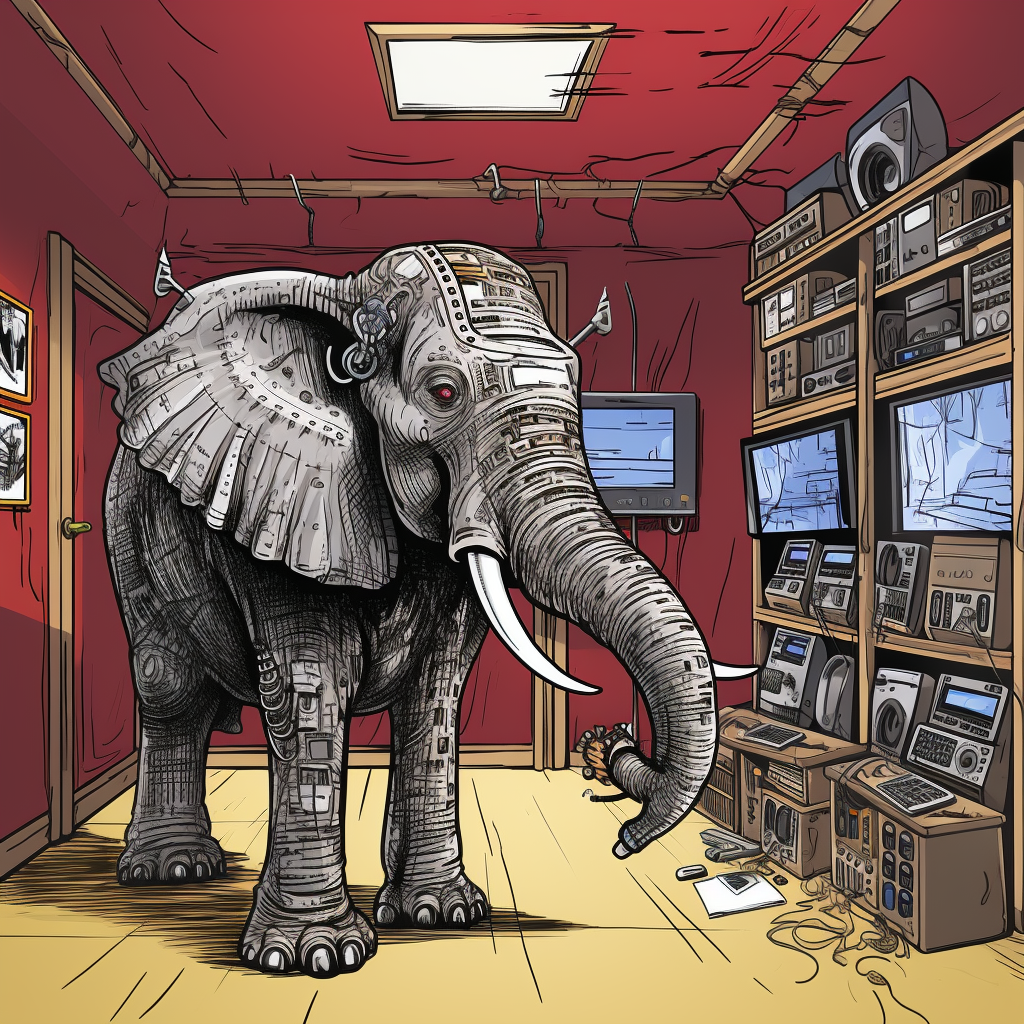
\includegraphics[width=0.4\linewidth]{../../img/ElefantInTheRoom} \end{center}

\begin{Shaded}
\begin{Highlighting}[]
\CommentTok{\# the symbolic representation of Artificial Intelligence as being the }
\CommentTok{\# "elefant in the room", comic cartoon style {-} Variations (Strong) }
\end{Highlighting}
\end{Shaded}
\end{block}

\begin{block}{Course concept}
\protect\hypertarget{course-concept}{}
\begin{itemize}
\item
  Learning mode in this course: Prepare with reading, visit the lecture,
  recap key concepts in lecture notes (self-study), work on exercises,
  watch solution video, come to exercise session, repeat\ldots{}
\item
  Strongly encouraged: (virtual) learning groups!

  \begin{itemize}
  \tightlist
  \item
    Biweekly exercises provide opportunity.
  \item
    Tackle the tricky exercises together!
  \end{itemize}
\end{itemize}
\end{block}

\begin{block}{Course concept: exercise sessions}
\protect\hypertarget{course-concept-exercise-sessions}{}
\begin{itemize}
\tightlist
\item
  In-class exercise sessions (bi-weekly evening sessions)

  \begin{itemize}
  \tightlist
  \item
    Discussion of exercises and additional input
  \item
    Recap of concepts
  \item
    Q\&A, support
  \item
    time for more coding!
  \end{itemize}
\end{itemize}
\end{block}

\begin{block}{Part I: Data (Science) fundamentals}
\protect\hypertarget{part-i-data-science-fundamentals}{}
\begin{longtable}[]{@{}ll@{}}
\toprule
Date & Topic \\
\midrule
\endhead
21.09.2023 & Introduction: Big Data/Data Science, course overview \\
28.09.2023 & Programming with R \\
05.10.2023 & An introduction to data and data processing \\
05.10.2023 & Exercises/Workshop 1: Tools, programming \\
12.10.2023 & Data storage and data structures \\
12.10.2023 & Exercises/Workshop 2: Data storage and data structures \\
19.10.2023 & Web data, text, and images \\
26.10.2023 & Data sources, data gathering, data import \\
26.10.2023 & Exercises/Workshop 3: Web data, text, and images \\
\bottomrule
\end{longtable}
\end{block}

\begin{block}{Part II: Data gathering and preparation}
\protect\hypertarget{part-ii-data-gathering-and-preparation}{}
\begin{longtable}[]{@{}
  >{\raggedright\arraybackslash}p{(\columnwidth - 2\tabcolsep) * \real{0.1209}}
  >{\raggedright\arraybackslash}p{(\columnwidth - 2\tabcolsep) * \real{0.8791}}@{}}
\toprule
\begin{minipage}[b]{\linewidth}\raggedright
Date
\end{minipage} & \begin{minipage}[b]{\linewidth}\raggedright
Topic
\end{minipage} \\
\midrule
\endhead
16.11.2023 & Data preparation and manipulation \\
23.11.2023 & Basic statistics and data analysis with R \\
23.11.2023 & Exercises/Workshop 4: Data gathering, data import \\
30.11.2023 & Guest Lecture: Matteo Courthoud (Senior Economist and Data
Scientist @Zalando) \\
\bottomrule
\end{longtable}
\end{block}

\begin{block}{Part III: Analysis, visualisation, output}
\protect\hypertarget{part-iii-analysis-visualisation-output}{}
\begin{longtable}[]{@{}
  >{\raggedright\arraybackslash}p{(\columnwidth - 2\tabcolsep) * \real{0.1028}}
  >{\raggedright\arraybackslash}p{(\columnwidth - 2\tabcolsep) * \real{0.8972}}@{}}
\toprule
\begin{minipage}[b]{\linewidth}\raggedright
Date
\end{minipage} & \begin{minipage}[b]{\linewidth}\raggedright
Topic
\end{minipage} \\
\midrule
\endhead
07.12.2023 & Visualisation, dynamic documents \\
07.12.2023 & Exercises/Workshop 5: Data preparation and applied data
analysis with R \\
14.12.2023 & Guest Lecture: Florian Chatagny (Head of Data Science
@Federal Finance Administration in Bern) \\
21.12.2023 & Exercises/Workshop 6: Visualization, dynamic documents \\
21.12.2023 & Summary, Wrap-Up, Q\&A, Feedback \\
21.12.2023 & Exam for Exchange Students \\
\bottomrule
\end{longtable}
\end{block}

\begin{block}{Core course resources}
\protect\hypertarget{core-course-resources}{}
\begin{itemize}
\tightlist
\item
  All information and materials (notes, slides, course sheet, syllabus,
  etc.) are available on StudyNet/Canvas.
\item
  Core materials will also be made available on Nuvolos.
\end{itemize}
\end{block}

\begin{block}{Main textbooks}
\protect\hypertarget{main-textbooks}{}
\href{https://umatter.github.io/datahandling/}{Data Handling Pocket
Reference}

\href{https://www.stat.auckland.ac.nz/~paul/ItDT/}{Murrell, Paul (2009).
\emph{Introduction to Data Technologies}, London: Chapman \& Hall/CRC.}

\href{http://r4ds.had.co.nz/}{Wickham, Hadley and Garred Grolemund
(2017). \emph{R for Data Science}, 1st Edition. Sebastopol, CA:
O'Reilly.}

\href{https://mdsr-book.github.io/mdsr3e/}{Baumer, Kaplan and Norton
(2023). \emph{Modern Data Science with R}, 2nd Edition.}
\end{block}

\begin{block}{Further resources}
\protect\hypertarget{further-resources}{}
\begin{itemize}
\tightlist
\item
  \href{https://stackoverflow.com/questions}{Stackoverflow}
\item
  \href{https://www.r-bloggers.com}{Get inspired in the R blogsphere}
\item
  ChatGPT
\end{itemize}
\end{block}

\begin{block}{Exam information}
\protect\hypertarget{exam-information}{}
\begin{itemize}
\tightlist
\item
  Central, written examination: \emph{digital, BYOD!}, we will have an
  instructional session by the head of the digital examinations team
  (data TBD).
\item
  Multiple choice questions.
\item
  A few open questions.
\item
  Theoretical concepts and practical applications in R (questions based
  on code examples).
\end{itemize}
\end{block}

\begin{block}{Exam information II}
\protect\hypertarget{exam-information-ii}{}
\begin{itemize}
\tightlist
\item
  We will release samples of multiple choice questions via Quizzes on
  Canvas/Studynet (exact same format and style of exam questions).
\item
  Exchange students who need to take the exam before the central exam
  block:

  \begin{itemize}
  \tightlist
  \item
    Date, time place, : \emph{21.12.2023, 16:15-18:00, room tbd}.
  \item
    Questions:
    \emph{\href{mailto:matthias.roesti@unisg.ch}{\nolinkurl{matthias.roesti@unisg.ch}}}
  \end{itemize}
\end{itemize}
\end{block}

\begin{block}{And now this\ldots{}}
\protect\hypertarget{and-now-this}{}
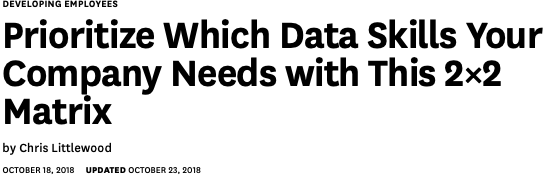
\includegraphics{../../img/ds_matrix.png}
\end{block}
\end{frame}

\begin{frame}{Q\&A}
\protect\hypertarget{qa}{}
\begin{block}{References}
\protect\hypertarget{references}{}
\end{block}
\end{frame}

\end{document}
